
\documentclass[xcolor={usenames,dvipsnames},10pt,compress]{beamer}

\usepackage[utf8]{inputenc}
\usepackage[english]{babel}
\usepackage{verbatim}
\usepackage{graphicx}
\usepackage{xspace}
\usepackage{amsthm}
\usepackage{url}
\usepackage{array}
\usepackage{hyperref}
\usepackage{times,mathptmx}
\usepackage{pdfpages}
\usepackage{mdframed}
\usepackage{tikz}
\usepackage{alltt}
%\usepackage[usenames,dvipsnames]{xcolor}
%\usepackage[usenames,dvipsnames]{color}
%\usepackage{color}

\usetikzlibrary{arrows,shapes}

\usetheme{Madrid}
%\usetheme{Boadilla}
%\usetheme{Darmstadt}
%\usetheme{Frankfurt}
%\usetheme{CambridgeUS}
%\usetheme{AnnArbor}
%\usecolortheme{beaver}
%\usecolortheme{seahorse}
%\usecolortheme{seagull}
\usecolortheme[named=BrickRed]{structure}

\setbeamercovered{transparent}

\setbeamertemplate{footline}[frame number]
%\setbeamertemplate{navigation symbols}{}
%\setbeamersize{text margin left=1em,text margin right=1em}

\newcommand{\titulo}{Programação Paralela com OpenMP}
\newcommand{\disciplina}{ELC139 - Programação Paralela}
\newcommand{\nome}{João Vicente Ferreira Lima (UFSM)}

\newcommand{\minicurso}{Interfaces de programação paralela com suporte a dependência de dados}
\newcommand{\tutorial}{Parallel programming interfaces for data-flow task programming}
\newcommand{\evento}{WSCAD 2014}
%\newcommand{\nome}{João Vicente Ferreira Lima (UFSM)}

\lecture[1]{\aula}{aula01}
\def\lecturename{\aula}

\newcommand{\Red}[1]{{\color{red}#1}}
\newcommand{\red}[1]{{\color{red}#1}}
\newcommand{\Blue}[1]{{\color{blue}#1}}
\newcommand{\blue}[1]{{\color{blue}#1}}

\newcommand{\PBS}[1]{\let\temp=\\#1\let\\=\temp}
\newcommand{\RRCOL}{\PBS\raggedright\hspace{0pt}}

\newcommand{\p}[1]{\texttt{#1}}
\newenvironment{code}{%
  \begin{alltt}%
  }{%
  \end{alltt}%
}

\makeatletter
%\setbeamertemplate{headline}{}
% {%
%   \leavevmode%
%   \@tempdimb=2.4375ex%
%   \ifnum\beamer@subsectionmax<\beamer@sectionmax%
%     \multiply\@tempdimb by 4%
%   \else%
%     \multiply\@tempdimb by\beamer@subsectionmax%
%   \fi%
%   \ifdim\@tempdimb>0pt%
%     \advance\@tempdimb by 1.125ex%
%     \begin{beamercolorbox}[wd=.5\paperwidth,ht=\@tempdimb]{section in head/foot}%
%       \vbox to\@tempdimb{\vfil\insertsectionnavigation{.5\paperwidth}\vfil}%
%     \end{beamercolorbox}%
%     \begin{beamercolorbox}[wd=.45\paperwidth,ht=\@tempdimb]{subsection in head/foot}%
%       \vbox
%       to\@tempdimb{\vfil\insertsubsectionnavigation{.45\paperwidth}\vfil}%
%     \end{beamercolorbox}%
%     \begin{beamercolorbox}[wd=.05\paperwidth,ht=\@tempdimb]{subsection in head/foot}%
%       \vbox
%       to\@tempdimb{\vfil\hfil\insertframenumber\vfil\vfil}%
%     \end{beamercolorbox}%
%   \fi%
% }

\def\dohead{\beamer@headcounter=4\relax\beamer@headcounter=1\loop\ifnum\beamer@headcounter<\beamer@totalheads%
  \advance\beamer@headcounter by1\relax%
  \csname @@head\the\beamer@headcounter\endcsname\repeat}

\makeatother

\title[\titulo]{\titulo}

\subtitle{\disciplina}

\author[João V. F. Lima]{\nome}

\institute[UFSM]{Universidade Federal de Santa Maria \\ \url{jvlima@inf.ufsm.br} \\ \url{http://www.inf.ufsm.br/~jvlima}}
\date{2023/1}

\graphicspath{{.}{figs/}}

\logo{ 
\includegraphics[height=1.5cm,width=1.5cm,keepaspectratio]{logo_inf}    
        
\includegraphics[height=1.5cm,width=1.5cm,keepaspectratio]{logo_ufsm} }

\newtheorem{mydef}{Definição}[section]
%\newtheorem{myteo}{Teorema}[section]
%------------------------------------------------------------------------------
\newcommand{\xkaapi}{XKaapi\xspace}
\newcommand{\kaapi}{KAAPI\xspace}
\newcommand{\kaapixx}{Kaapi++\xspace}
%------------------------------------------------------------------------------
% Typesetting Listings
\usepackage{listings}
\lstset{
  language=C,
  %basicstyle=\scriptsize\ttfamily,
  %basicstyle=\normalsize\ttfamily,
  %basicstyle=\small\ttfamily,
  basicstyle=\footnotesize\ttfamily,
  aboveskip=0pt,
  belowskip=0pt,
  mathescape=false,
  columns=flexible,
  numbers=none,
%  showtabs=true,
%  showspaces=true,
  breaklines=true
}
%------------------------------------------------------------------------------
\lstset{commentstyle=\color{blue}}
%\lstset{stringstyle=\ttfamily}
\lstset{ classoffset=1, 
            morekeywords={kaapi,omp,task,data,alloca, declare, reduction, identity, parallel,sync,taskwait,cilk,spawn,tbb,css,cilk\_spawn,cilk\_sync,cilk\_for,offload},
            keywordstyle=\color{Red}\bfseries
           }
\lstset{ classoffset=2, 
            morekeywords={value,read,write,readwrite,reduction,untied,firstprivate,TaskBodyCPU,TaskBodyGPU,ka,Signature,RW,CW,range2d\_r,range2d\_rw,range2d,Spawn,Fork,Shared\_w,Shared\_r,Shared,a1,target,device,copyin,copyout,input,implements,copy\_deps,RPWP,range2d\_rpwp,rangeindex,Memory,Register,SetStaticSched,Sync,Unregister,Community,System,join\_community,SpawnMain,leave,initialize,terminate,logfile,array,SetArch,ArchHost,ArchCUDA,W,R,gpuStream,pointer\_w,pointer\_r,pointer\_cw,pointer},
            keywordstyle=\color{Blue}\bfseries
           }
\lstset{ classoffset=3, 
            morekeywords={storage,ld},
            keywordstyle=\bfseries
           }
\lstset{ classoffset=4, 
            morekeywords={in,out,inout,cout,concurrent},
            keywordstyle=\color{Red}\bfseries
           }
           
\lstset{classoffset=0, showstringspaces=false}
%------------------------------------------------------------------------------
\mdfsetup{
  backgroundcolor=gray!10,
%  roundcorner=10pt,
}
%------------------------------------------------------------------------------

\begin{document}

\begin{frame}
%  \titlepage
  \maketitle
\end{frame}

\begin{frame}
    \frametitle{Outline}
    \tableofcontents[hideallsubsections]
%    \tableofcontents
\end{frame}

\AtBeginSection{
  \begin{frame}
    \frametitle{Outline}
    \tableofcontents[currentsection,hideothersubsections]
  \end{frame}
}

%
%%%%%%%%%%%%%%%%%%%%%%%%%%%%%%%%%%%%%%%%%%%%%%%%%%%%%%%%%%%%%%%%%%%%%%%%%%%%%%%
%\section*{Palestrantes}
%%%%%%%%%%%%%%%%%%%%%%%%%%%%%%%%%%%%%%%%%%%%%%%%%%%%%%%%%%%%%%%%%%%%%%%%%%%%%%%

%------------------------------------------------------------------------------
\begin{frame}
  \frametitle{Palestrante}
  {\bf Prof. João V. F. Lima (UFSM)}
  \begin{itemize}
  \item (2014-autal) Professor na Universidade Federal de Santa Maria (UFSM)
  \item Áreas de atuação
    \begin{itemize}
    \item Processamento de Alto Desempenho
    \item Programação Paralela
    \item Linguagens de Programação
    \end{itemize}
  \end{itemize}
\end{frame}
%------------------------------------------------------------------------------
\begin{frame}[fragile]
  \frametitle{Sobre o Minicurso}
  \begin{itemize}
  \item Partes deste minicurso
    \begin{description}
    \item[Parte I] -- Introdução em arquiteturas e programação
    \end{description}
  \item Pré-requisitos
    \begin{itemize}
    \item Linguagem C
    \item Programação paralela (básico)
    \end{itemize}
  \end{itemize}
  %
  \begin{block}{Exemplos no GitHub:}
\begin{lstlisting}[basicstyle=\footnotesize\ttfamily,language=,numbers=none]
git clone https://github.com/joao-lima/wscad-2014-minicurso.git
\end{lstlisting}
  \end{block}
\end{frame}

%%%%%%%%%%%%%%%%%%%%%%%%%%%%%%%%%%%%%%%%%%%%%%%%%%%%%%%%%%%%%%%%%%%%%%%%%%%%%%%%
\section{Introduction}
%%%%%%%%%%%%%%%%%%%%%%%%%%%%%%%%%%%%%%%%%%%%%%%%%%%%%%%%%%%%%%%%%%%%%%%%%%%%%%%
%------------------------------------------------------------------------------
\begin{frame}
  \frametitle{Introduction}
  \begin{itemize}
  \item Widespread usage of multicores and accelerators.
    \begin{itemize}
    \item Highly parallel computing units.
    \item Energy-efficient and low cost devices.
    \end{itemize}

  \item Many applications take advantage of parallel architectures.
  \end{itemize}
  %
  \begin{center}
    \begin{figure}
      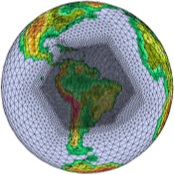
\includegraphics[width=2cm]{olam}
      \hspace{2mm}
      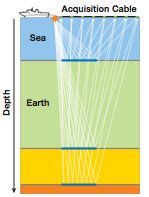
\includegraphics[width=2cm]{seismic}
      \hspace{2mm}
      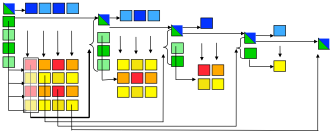
\includegraphics[width=3cm]{fig-lu}
    \end{figure}
  \end{center}
  %
  \begin{itemize}
  \item {\bf Asynchronicity and fine granularity are essential}.
    \begin{itemize}
    \item Avoid/loose synchronizations.
    \item Improve load balancing.
    \item Exploit the available parallelism.
    \end{itemize}
  \end{itemize}
\end{frame}
%------------------------------------------------------------------------------
\begin{frame}
  \frametitle{Introduction}
  \begin{itemize}
  \item {\bf Runtime} - abstraction of the underlying architecture.
    \begin{itemize}
    \item View of parallelism.
    \item View of memory.
    \end{itemize}
  \end{itemize}
  %
  \begin{figure}
  \centering
  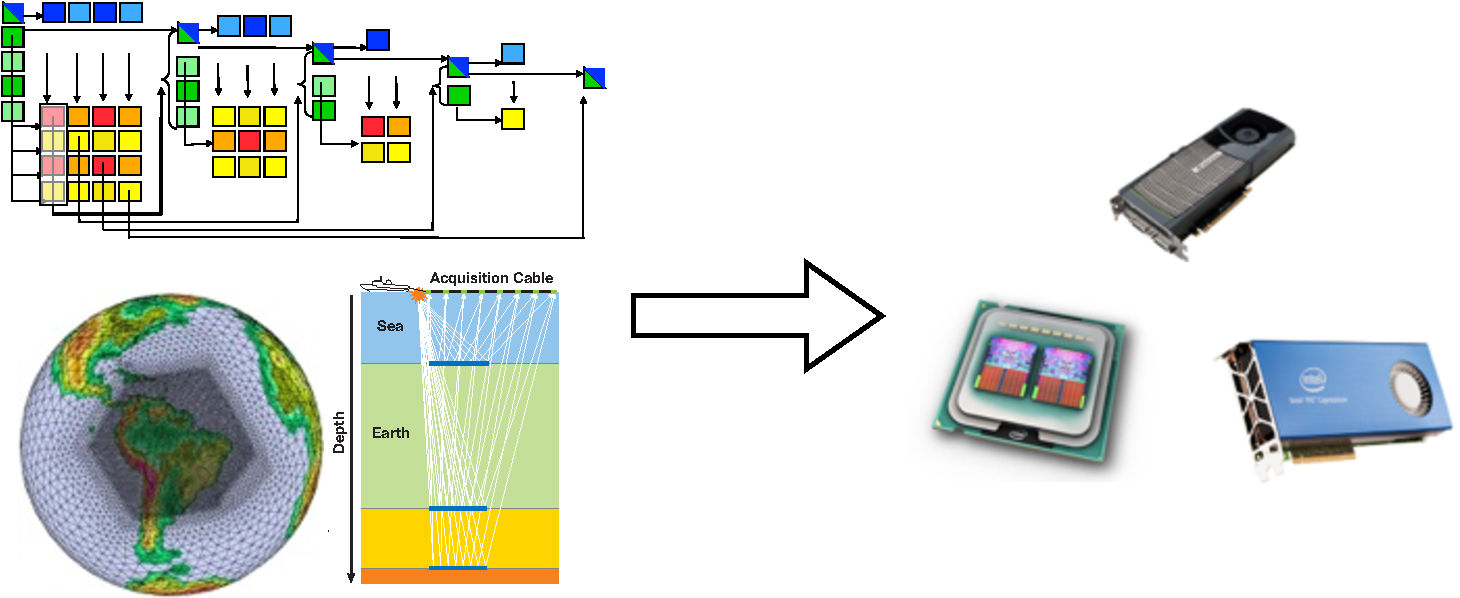
\includegraphics[width=0.8\textwidth]{runtime-system-crop}
  \end{figure}
  %
  \begin{itemize}
  \item {\large In this tutorial we study {\bf data-flow task programming} interfaces.}
  \end{itemize}
\end{frame}
%------------------------------------------------------------------------------
\begin{frame}
  \frametitle{Introduction}
  \begin{exampleblock}{Data-flow task programming}
    Combination of \alert<2->{parallelism} and \alert<2->{memory} view.
    \begin{itemize}
    \item Parallelism is explicit.
    \item Memory view is implicit and \alert<2->{synchronization relies on the runtime}.
    \end{itemize}
  \end{exampleblock}
  %
  \begin{itemize}
  \item Popular in heterogeneous systems.
    \begin{itemize}
    \item A way to express the memory view on disjoint address spaces.
    \end{itemize}
  \item First ``modern'' applications: \blue{tiled algorithms on multicore systems}.
    \begin{itemize}
    \item PLASMA/QUARK from UTK.
    \end{itemize}
  \item Well studied since 1998 with Athapascan/KAAPI (Grenoble/France).
    \begin{itemize}
    \item Now XKaapi.
    \end{itemize}
  \end{itemize}
\end{frame}
%------------------------------------------------------------------------------

%%%%%%%%%%%%%%%%%%%%%%%%%%%%%%%%%%%%%%%%%%%%%%%%%%%%%%%%%%%%%%%%%%%%%%%%%%%%%%%
\section{Task parallelism}
%%%%%%%%%%%%%%%%%%%%%%%%%%%%%%%%%%%%%%%%%%%%%%%%%%%%%%%%%%%%%%%%%%%%%%%%%%%%%%%
%%%%%%%%%%%%%%%%%%%%%%%%%%%%%%%%%%%%%%%%%%%%%%%%%%%%%%%%%%%%%%%%%%%%%%%%%%%%%%%
\subsection{Task parallelism}
%------------------------------------------------------------------------------
\begin{frame}
  \frametitle{Task parallelism}
  \begin{block}{Task parallelism}
    \begin{itemize}
    \item {\bf Task parallelism} or \blue{functional parallelism} or \blue{control parallelism}.
    \item Decomposes the \red{computation} rather than the \red{manipulated data}.
      \begin{itemize}
      \item Programming model for tasks that perform different computations.
      \end{itemize}
    \item Ex.: Cilk, Intel TBB, OpenMP.
    \end{itemize}
  \end{block}
  %
  \pause
  %
  \begin{exampleblock}{Task dependency}
    \begin{itemize}
    \item Tasks with dependencies can unfold a \red{directed acyclic graph} (DAG).
      \begin{itemize}
      \item Expressed by synchronization such as \texttt{sync} keyword.
      \end{itemize}
    \item If data dependencies are considered, the algorithm unfolds a \red{data flow graph} (DFG).
    \item Ex.: Jade, Athapascan, OpenMP (\red{new}), KAAPI/XKaapi, StarPU, OmpSs, 
      Intel Offload.
    \end{itemize}
  \end{exampleblock}
\end{frame}
%------------------------------------------------------------------------------
%%%%%%%%%%%%%%%%%%%%%%%%%%%%%%%%%%%%%%%%%%%%%%%%%%%%%%%%%%%%%%%%%%%%%%%%%%%%%%%
%% \subsection{Intel Cilk Plus}
%% %------------------------------------------------------------------------------
%% \begin{frame}[fragile]
%%   \frametitle{Intel Cilk Plus}
%%   \begin{itemize}
%%   \item Extensions to C/C++ to support {\bf fork-join parallelism}.
%%     \begin{itemize}
%%     \item Based on Cilk (MIT) and Cilk++ (Cilk Arts).
%%     \end{itemize}
%%   \item Efficient work-stealing scheduler.
%%   \item Offers \blue{hyperobjects} (lock-free mechanism).
%%   \end{itemize}
%%   %
%%   \begin{exampleblock}{Cilk Plus keywords}
%%     \begin{itemize}
%%     \item \verb+cilk_spawn+ - asynchronous function call.
%%     \item \verb+cilk_sync+ - synchronization, must wait all spawned tasks.
%%     \item \verb+cilk_for+ - parallel iterations.
%%     \end{itemize}
%%   \end{exampleblock}
%% \end{frame}
%% %------------------------------------------------------------------------------
%% \begin{frame}[fragile]
%%   \frametitle{Intel Cilk Plus}
%%   \vspace{-4mm}
%%   \begin{columns}
%%     \begin{column}{0.5\textwidth}
%%   \begin{block}{Thread parallelism}
%% \begin{lstlisting}
%% main(void)
%% {
%%   cilk_spawn f();
%%   cilk_spawn g();
%%   // nop
%%   cilk_sync;
%% }
%% \end{lstlisting}
%%   \end{block}
%%     \end{column}
%%     %
%%     \begin{column}{0.5\textwidth}
%%       \begin{flushleft}
%% 	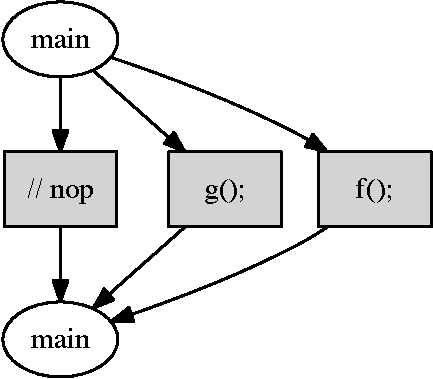
\includegraphics[width=\textwidth]{cilk-fork-1-crop}
%%       \end{flushleft}
%%     \end{column}
%%   \end{columns}
%% \end{frame}
%% %------------------------------------------------------------------------------
%% \begin{frame}[fragile]
%%   \frametitle{Intel Cilk Plus}
%%   \vspace{-4mm}
%%   \begin{columns}
%%     \begin{column}{0.5\textwidth}
%%   \begin{block}{Thread parallelism}
%% \begin{lstlisting}
%% main(void) 
%% {
%%   cilk_spawn f();
%%   g();
%%   // nop
%%   cilk_sync;
%% }
%% \end{lstlisting}
%%   \end{block}
%%     \end{column}
%%     %
%%     \begin{column}{0.5\textwidth}
%%       \begin{flushleft}
%% 	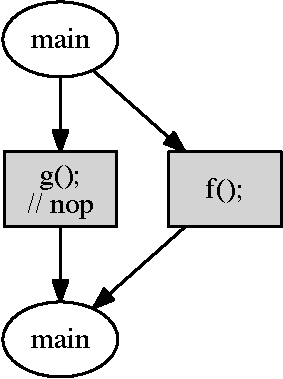
\includegraphics[width=0.7\textwidth]{cilk-fork-2-crop}
%%       \end{flushleft}
%%     \end{column}
%%   \end{columns}
%% \end{frame}
%% %------------------------------------------------------------------------------
%% \begin{frame}[fragile]
%%   \frametitle{Intel Cilk Plus}
%%   \begin{block}{Parallel loops}
%% \begin{lstlisting}
%% for( int i = 0; i < n; i++ )
%% {
%%   cilk_spawn do_work(i);
%% }
%% cilk_sync;
%% \end{lstlisting}
%%   \end{block}
%%   %
%%   \pause
%%   %
%%   \begin{exampleblock}{Parallel loops (divide-and-conquer)}
%% \begin{lstlisting}
%% cilk_for for( int i = 0; i < n; i++ )
%% {
%%   do_work(i);
%% }
%% \end{lstlisting}
%%   \end{exampleblock}
%% \end{frame}
%% %------------------------------------------------------------------------------
%% %%%%%%%%%%%%%%%%%%%%%%%%%%%%%%%%%%%%%%%%%%%%%%%%%%%%%%%%%%%%%%%%%%%%%%%%%%%%%%%
%% %\subsection{Intel TBB}
%% %------------------------------------------------------------------------------
%% %\begin{frame}
%% %  \frametitle{Intel Threading Building Blocks}
%% %\end{frame}
%------------------------------------------------------------------------------
%%%%%%%%%%%%%%%%%%%%%%%%%%%%%%%%%%%%%%%%%%%%%%%%%%%%%%%%%%%%%%%%%%%%%%%%%%%%%%%
\subsection{OpenMP}
%------------------------------------------------------------------------------
\begin{frame}[fragile]
  \frametitle{OpenMP tasks}
\begin{block}{Task construct}
\begin{lstlisting}
#pragma omp task
\end{lstlisting}
\end{block}
%
\pause
%
\begin{block}{Barrier \texttt{taskwait}}
\begin{lstlisting}
#pragma omp taskwait
\end{lstlisting}
\end{block}
%
\pause
%
\begin{itemize}
\item Independent units of work.
\item Recursive tasks.
\item Unfold parallelism at runtime.
\item The OpenMP implementation decides when/where to execute: 
  \begin{itemize}
  \item Immediately (in depth, \blue{depth-first} or \blue{work-first})
  \item Latter (in breadth, \blue{breadth-first} or \blue{help-first})
  \end{itemize}
\end{itemize}
%
\end{frame}
%------------------------------------------------------------------------------
\begin{frame}[fragile]
  \frametitle{OpenMP tasks}
\begin{block}{Linked list}
\begin{lstlisting}
node* p = head;
while(p) {
  process(p);
  p = p->next;
}
\end{lstlisting}
\end{block}
%
\end{frame}
%------------------------------------------------------------------------------
% \begin{frame}[fragile]
%   \frametitle{OpenMP tasks}
% \begin{block}{Linked list - parallel version}
% \begin{lstlisting}
% #pragma omp parallel
% {
% #pragma omp single 
%   {
%     node* p = head;
%     while(p) {
% #pragma omp task 
%       process(p);
%       p = p->next;
%     }
%   }
% }
% \end{lstlisting}
% \end{block}
% %
% \end{frame}
%------------------------------------------------------------------------------
\begin{frame}[fragile]
  \frametitle{OpenMP tasks}
\begin{block}{Linked list - parallel version}
\begin{lstlisting}
#pragma omp parallel
{
#pragma omp single 
  {
    node* p = head;
    while(p) {
#pragma omp task firstprivate(p)
      process(p);
      p = p->next;
    }
  }
}
\end{lstlisting}
\end{block}
%
\end{frame}
%------------------------------------------------------------------------------
\begin{frame}[fragile]
  \frametitle{OpenMP tasks}
\begin{block}{Cálculo de Fibonacci}
\begin{lstlisting}
int fib( int n ) {
  int x, y;
  if( n < 2 ) return n;
  x = fib( n - 1);
  y = fib( n - 2);
  return x + y;
}
\end{lstlisting}
\end{block}
%
\end{frame}
%------------------------------------------------------------------------------
\begin{frame}[fragile]
  \frametitle{Paralelismo de Tarefas}
\begin{block}{Cálculo de Fibonacci com OpenMP}
\begin{lstlisting}
int fib( int n ) {
  int x, y;
  if( n < 2 ) return n;
#pragma omp task
  x = fib( n - 1);
#pragma omp task
  y = fib( n - 2);
#pragma omp taskwait
  return x + y;
}
\end{lstlisting}
\end{block}
%
\onslide<2->
%
\begin{alertblock}{Correto?}
\onslide<3->{Não pois x e y são privados fora do escopo das tarefas.}
\end{alertblock}
%
\end{frame}
%------------------------------------------------------------------------------
\begin{frame}[fragile]
  \frametitle{Paralelismo de Tarefas}
\begin{block}{Cálculo de Fibonacci com OpenMP}
\begin{lstlisting}
int fib( int n ) {
  int x, y;
  if( n < 2 ) return n;
#pragma omp task shared(x)
  x = fib( n - 1);
#pragma omp task shared(y)
  y = fib( n - 2);
#pragma omp taskwait
  return x + y;
}
\end{lstlisting}
\end{block}
%
\begin{exampleblock}{Agora sim}
Necessitamos dos dois valores no cálculo.
\end{exampleblock}
%
\end{frame}
%------------------------------------------------------------------------------

%%%%%%%%%%%%%%%%%%%%%%%%%%%%%%%%%%%%%%%%%%%%%%%%%%%%%%%%%%%%%%%%%%%%%%%%%%%%%%%
\section{Data flow dependency}
%%%%%%%%%%%%%%%%%%%%%%%%%%%%%%%%%%%%%%%%%%%%%%%%%%%%%%%%%%%%%%%%%%%%%%%%%%%%%%%
%------------------------------------------------------------------------------
%%%%%%%%%%%%%%%%%%%%%%%%%%%%%%%%%%%%%%%%%%%%%%%%%%%%%%%%%%%%%%%%%%%%%%%%%%%%%%%
\subsection{Data flow dependency}
%------------------------------------------------------------------------------
\begin{frame}
  \frametitle{Data flow dependency}
  \begin{block}{Concept}
    Similar to a DAG of tasks, but combines {\bf task dependencies with data-driven execution}.
    \begin{itemize}
    \item Execution is controlled by the {\bf Data Flow Graph (DFG)}.
    \item Unlike the program recursion structure of {\bf full strict model}.
    \end{itemize}
  \end{block}
  %
  \vspace{-4mm}
  %
  \begin{columns}
    \begin{column}{0.5\textwidth}
      \begin{center}
	{\bf Fully strict mode (Cilk)}
      \end{center}
    \end{column}
    %
    \begin{column}{0.5\textwidth}
      \begin{center}
	{\bf Data flow graph}
      \end{center}
    \end{column}
  \end{columns}
  %
  \vspace{-2mm}
  %
  \begin{columns}
    \begin{column}{0.5\textwidth}
      \begin{center}
	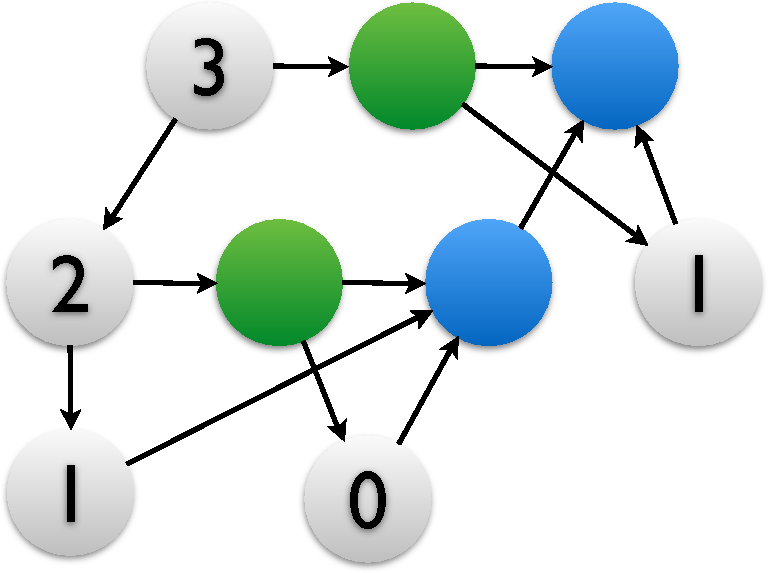
\includegraphics[width=0.8\textwidth]{dag-strict-crop}
      \end{center}
    \end{column}
    %
    \begin{column}{0.5\textwidth}
      \begin{center}
	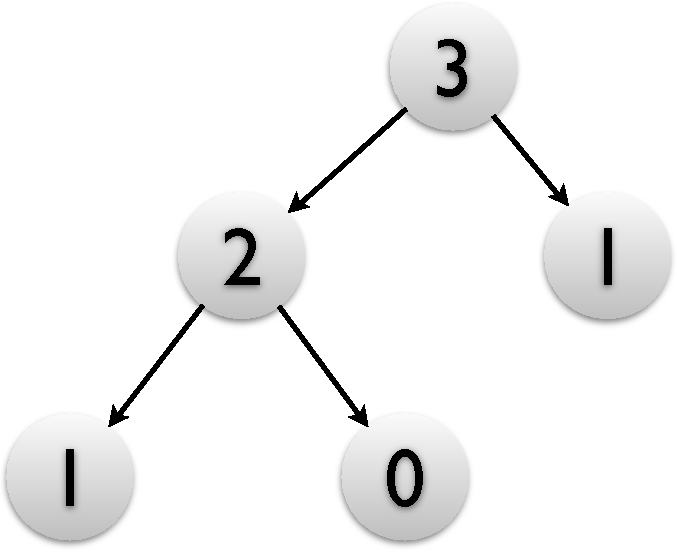
\includegraphics[width=0.8\textwidth]{dag-dfg-crop}
      \end{center}
    \end{column}
  \end{columns}
\end{frame}
%------------------------------------------------------------------------------
\begin{frame}
  \frametitle{Data flow dependency}
  \begin{exampleblock}{Data access modes}
    \begin{itemize}[<+->]
    \item \blue{Read only}  ({\bf RO or R}) - only read, no permission to modify.
    \item \blue{Write only}  ({\bf WO or W}) - only write, no wait for data inputs.
    \item \blue{Read and Write} ({\bf RW}) - or exclusive mode, read and write.
    \item \blue{Cumulative Write} ({\bf CW}) - concurrent write and cumulative.
    \end{itemize}
  \end{exampleblock}
\end{frame}
%------------------------------------------------------------------------------
\begin{frame}[fragile]
  \frametitle{Data flow dependency}
  The concepts here \red{are the same} from \blue{computer architecture} in which
  we can replace {\bf instruction} by {\bf task}.
  %
  \begin{block}{Data dependencies}
    \begin{itemize}
    \item Task $t_i$ produces a result that may be used by a task $t_j$.
    \item Task $t_j$ is data dependent on task $t_k$, and $t_k$ is 
    data dependent on $t_i$ ($t_i \rightarrow t_k \rightarrow t_j$). 
    \end{itemize}
  \end{block}
  %
  \vspace*{-4mm}
  %
  \begin{columns}
  \begin{column}{0.6\textwidth}
  \begin{flushright}
  \begin{block}{}
\begin{lstlisting}
compute( input, &result );

display( &result );
\end{lstlisting}
  \end{block}
  \end{flushright}
  \end{column}
  %
    \begin{column}{0.4\textwidth}
      \begin{flushleft}
	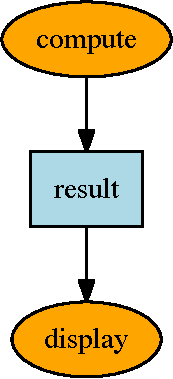
\includegraphics[width=0.4\textwidth]{dependency-crop}
      \end{flushleft}
    \end{column}
  \end{columns}
  %
\begin{tikzpicture}[overlay,>=stealth]
\draw<2-> [->,line width=2pt,red] (2.9, 2.6) .. controls(2.4, 2.2) .. (1.9, 2) node {};
\end{tikzpicture}
\end{frame}
%------------------------------------------------------------------------------
%\begin{frame}
%  \frametitle{Flow dependency}
%  \begin{exampleblock}{Flow dependency}
%    Ou dependência de dados, \emph{data dependency}, \emph{true dependency}, ou 
%    \textbf{read-after-write (RAW)} onde uma tarefa depende do resultado produzido
%    por uma tarefa anterior.
%  \end{exampleblock}
%  \begin{center}
%    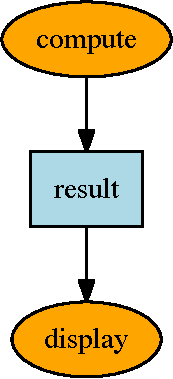
\includegraphics[scale=0.6]{dependency-crop}
%  \end{center}
%\end{frame}
%------------------------------------------------------------------------------
\begin{frame}
  \frametitle{Data hazards}
  \begin{alertblock}{Data hazards}
  There is a \textbf{dependence} between task and the we must preserve the execution order. 
  %
    \begin{itemize}
    \item \textbf{RAW} (\emph{Read after Write}).
    \item \textbf{WAW} (\emph{Write after Write}).
    \item \textbf{WAR} (\emph{Write after Read}).
    \end{itemize}
  \end{alertblock}
  %
\end{frame}
%------------------------------------------------------------------------------
%------------------------------------------------------------------------------
%------------------------------------------------------------------------------
\begin{frame}
  \frametitle{Data flow dependency}
%  \vspace*{-4cm}
  \begin{columns}
  \begin{column}{0.4\textwidth}
	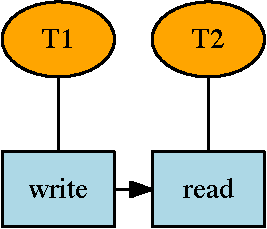
\includegraphics[width=\textwidth]{read-after-write-crop}
  \end{column}
  %
  \begin{column}{0.6\textwidth}
    \begin{itemize}
    \item \textbf{RAW} (\emph{Read after Write}) - or \blue{true dependency}, \blue{data dependency}.
    \item A task depends on the result produced by a previous task.
    \end{itemize}
  \end{column}
  \end{columns}
\end{frame}
%------------------------------------------------------------------------------
\begin{frame}
  \frametitle{Data flow dependency}
  \begin{columns}
  \begin{column}{0.4\textwidth}
	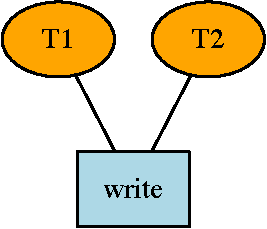
\includegraphics[width=\textwidth]{write-after-write-crop}
  \end{column}
  %
  \begin{column}{0.6\textwidth}
    \begin{itemize}
    \item \textbf{WAW} (\emph{Write after Write}) - or \blue{output dependency}.
    \item The execution order will affect the final output.
    \end{itemize}
  \end{column}
  \end{columns}
\end{frame}
%------------------------------------------------------------------------------
\begin{frame}
  \frametitle{Data flow dependency}
  \begin{columns}
  \begin{column}{0.4\textwidth}
	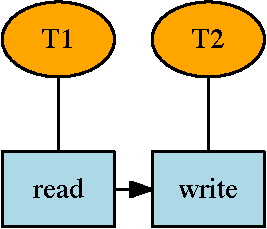
\includegraphics[width=\textwidth]{write-after-read-crop}
  \end{column}
  %
  \begin{column}{0.6\textwidth}
    \begin{itemize}
    \item \textbf{WAR} (\emph{Write after Read}) - or \blue{anti-dependency}.
    \item A task writes a value before it is read.
    \end{itemize}
  \end{column}
  \end{columns}
\end{frame}
%------------------------------------------------------------------------------
%%%%%%%%%%%%%%%%%%%%%%%%%%%%%%%%%%%%%%%%%%%%%%%%%%%%%%%%%%%%%%%%%%%%%%%%%%%%%%%
\subsection{Data flow example}
%------------------------------------------------------------------------------
\begin{frame}[fragile]
  \frametitle{Data flow example}
  In our next examples, we will use the following keywords:
  \begin{itemize}
  \item \textbf{in} - read access.
  \item \textbf{out} - write access.
  \item \textbf{inout} - read and write access.
  \end{itemize}
  %
\begin{block}{}
\begin{lstlisting}
void reading(in int a) {}
void modifying(inout int b) {}
main(void)
{
  int a;
  reading( a );
  reading( a );
  reading( a );
  modifying( a );
  modifying( a );
}
\end{lstlisting}
\end{block}
%  \begin{code}\footnotesize
%void reading(in int a)
%\{
%  \emph{\color{OliveGreen}{/* code here */}}
%\}
%void modifying(inout int b)
%\{
%  \emph{\color{OliveGreen}{/* code here to modify data */}}
%\}
%main(void)
%\{
%  int a;
%  reading( a );
%  reading( a );
%  reading( a );
%  modifying( a );
%  modifying( a );
%\}
%  \end{code}
\end{frame}
%------------------------------------------------------------------------------
\begin{frame}[fragile]
  \frametitle{Data flow example}
  \begin{columns}
  \begin{column}{0.6\textwidth}
\begin{block}{}
\begin{lstlisting}[escapeinside={@}{@}]
void reading(in int a) {}
void modifying(inout int b) {}
main(void)
{
  int a;
  @\alert<2>{reading( a );}@
  @\alert<3>{reading( a );}@
  @\alert<4>{reading( a );}@
  @\alert<5>{modifying( a );}@
  @\alert<6>{modifying( a );}@
}
\end{lstlisting}
%  @{\bfseries\color{Red}{modifying( a );}}@
\end{block}
  \end{column}
  \begin{column}{0.4\textwidth}
  \hspace{10mm}
  \begin{tikzpicture}[node distance=1.5cm,overlay,>=stealth]
  \tikzstyle{task}=[shape=circle,draw,thick,inner sep=0pt,minimum size=25pt,draw=black,fill=blue!20]
  \tikzstyle{mode}=[shape=rectangle,draw,thick,inner sep=0pt,minimum size=30pt,draw=black,fill=red!20]
  \node<2-> [task] (t1) {{\large$t_1$}};
  \node<2-> [task] (t2) [below of=t1] {{\large$t_2$}};
  \node<2-> [task] (t3) [below of=t2] {{\large$t_3$}};
  \node<2-> [mode] (m1) [right of=t2] {{\large\bf R}};
  \path<2-> (m1) edge [thick] (t1);
  \path<3-> (m1) edge [thick] (t2);
  \path<4-> (m1) edge [thick] (t3);
  %
  \node<5-> [task] (t4) [below of=t3] {{\large$t_4$}};
  \node<5-> [mode] (m2) [right of=t4] {{\large\bf RW}};
  \path<5-> (m2) edge [thick] (t4);
  \path<5-> (m2) edge [<-,thick] (m1);
  %
  \node<6-> [task] (t5) [below of=t4] {{\large$t_5$}};
  \node<6-> [mode] (m3) [right of=t5] {{\large\bf RW}}
    edge [thick] (t5)
    edge [<-,thick] (m2);
  \end{tikzpicture}
  \vspace{60mm}
  \end{column}
  \end{columns}
\end{frame}
%------------------------------------------------------------------------------
%------------------------------------------------------------------------------
%------------------------------------------------------------------------------
\begin{frame}[fragile]
  \frametitle{Fibonacci example}
\begin{block}{}
\begin{lstlisting}
void fibo( int n, int* res )
{
  int x, y;
  if( n < 2 ){
    *res = n;
  } else {
    fibo( n-1, &x );
    fibo( n-2, &y );
    *res = x+y;
  }
}

int main(void) {
  int n = 3, res;
  fibo( n, &res );
  print( res );
  return 0;
}
\end{lstlisting}
\end{block}
\end{frame}
%------------------------------------------------------------------------------
\begin{frame}[fragile]
  \frametitle{Fibonacci example}
  \begin{alertblock}{Notice}
    This recursive Fibonacci is not the best implementation, but it serves our purposes.
  \end{alertblock}
  %
  \pause
  %
  \begin{exampleblock}{Dependency example (again)}
    In our next example, we will use the following keywords:
    \begin{itemize}
    \item \textbf{in} - read access.
    \item \textbf{out} - write access.
    \item \textbf{inout} - read and write access.
    \item \textbf{cout} - cumulative write with global reduction.
    \end{itemize}
  \end{exampleblock}
\end{frame}
%------------------------------------------------------------------------------
\begin{frame}[fragile]
  \frametitle{Fibonacci example}
\begin{block}{}
\begin{lstlisting}
void fibo( in int n, out int* res )
{
  int x, y;
  if( n < 2 ){
    *res = n;
  } else {
    fibo( n-1, &x );
    fibo( n-2, &y );
    *res = x+y;
  }
}

int main(void) {
  int n = 3, res;
  fibo( n, &res );
  print( res );
  return 0;
}
\end{lstlisting}
\end{block}
%
\begin{tikzpicture}[overlay,>=stealth]
\draw<2-> [draw=red,very thick] (1.4,3.8) ellipse (30pt and 10pt);
\end{tikzpicture}
%
\end{frame}
%------------------------------------------------------------------------------
\begin{frame}[fragile]
  \frametitle{Fibonacci example}
\begin{block}{Previous Fibonacci example}
\begin{lstlisting}[firstnumber=6]
  } else {
    fibo( n-1, &x );
    fibo( n-2, &y );
    *res = x+y;
  }
\end{lstlisting}
\end{block}
%
\pause
%
\begin{alertblock}{Synchronization problem}
If our tasks execute in parallel, we would like \textbf{to wait} for the
results from the previous two \texttt{fibo} tasks.
\end{alertblock}
%
\pause
%
\begin{exampleblock}{Solution}
  \begin{enumerate}
  \item An explicit synchronization (Cilk's style).
  \item A task that depends on the results from the two \texttt{fibo} tasks.
  \end{enumerate}
\end{exampleblock}
%
\end{frame}
%------------------------------------------------------------------------------
\begin{frame}[fragile]
  \frametitle{Fibonacci example}
\begin{block}{}
\begin{lstlisting}
void sum( out int* res, in int x, in int y )
{
  *a = x + y;
}

void fibo( in int n, out int* res )
{
  int x, y;
  if( n < 2 ){
    *res = n;
  } else {
    fibo( n-1, &x );
    fibo( n-2, &y );
    sum( res, x, y );
  }
}
\end{lstlisting}
\end{block}
%
\begin{tikzpicture}[overlay,>=stealth]
\draw<2-> [draw=red,very thick] (1.8,1.5) ellipse (40pt and 10pt);
\end{tikzpicture}
%
\end{frame}
%------------------------------------------------------------------------------
\begin{frame}[fragile]
  \frametitle{Fibonacci example (cumulative)}
\begin{block}{}
\begin{lstlisting}
void fibo( in int n, cout int* res )
{
  int x, y;
  if( n < 2 ){
    *res += n;
  } else {
    fibo( n-1, &x );
    fibo( n-2, &y );
  }
}
\end{lstlisting}
\end{block}
%
\begin{tikzpicture}[overlay,>=stealth]
\draw<2-> [draw=red,very thick] (1.5,2.5) ellipse (30pt and 10pt);
\draw<2-> [draw=red,very thick] (3.8,3.9) ellipse (15pt and 10pt);
\end{tikzpicture}
%
\end{frame}
%------------------------------------------------------------------------------
%\begin{frame}
%  \frametitle{Data flow dependency}
%  \vspace*{-4cm}
%  \begin{tikzpicture}[node distance=1.5cm,overlay,>=stealth]
%  \tikzstyle{task}=[shape=circle,draw,thick,inner sep=0pt,minimum size=25pt,draw=black,fill=blue!20]
%  \tikzstyle{mode}=[shape=rectangle,draw,thick,inner sep=0pt,minimum size=30pt,draw=black,fill=red!20]
%%  \path[use as bounding box] (-1,0) rectangle(10,-2);
%  \node[task] (t1) {{\large$t_1$}};
%  \node[mode] (m1) [below of=t1] {{\large\bf RW}}
%    edge [thick] (t1);
%  %
%  \node[task] (t2) [right of=t1] {{\large$t_2$}};
%  \node[task] (t3) [right of=t2] {{\large$t_3$}};
%  \node[mode] (m2) [below of=t2] {{\large\bf R}}
%    edge [thick] (t2)
%    edge [thick] (t3)
%    edge [<-,thick] (m1);
%  %
%  \node[task] (t4) [right of=t3] {{\large$t_4$}};
%  \node[mode] (m3) [below of=t4] {{\large\bf W}}
%    edge [thick] (t4)
%    edge [<-,thick] (m2);
%  %
%  \node[task] (t5) [right of=t4] {{\large$t_5$}};
%  \node[task] (t6) [right of=t5] {{\large$t_6$}};
%  \node[task] (t7) [right of=t6] {{\large$t_7$}};
%  \node[mode] (m4) [below of=t6] {{\large\bf CW}}
%    edge [thick] (t5)
%    edge [thick] (t6)
%    edge [thick] (t7)
%    edge [<-,thick] (m3);
%  \node[task] (taa) [below of=m1] {{\large$t_i$}};
%  \node (ttaa) [right of=taa,right] {{\large Nó tarefa}};
%  \node[mode] (maa) [below of=taa] {{\large R}};
%  \node  [right of=maa,right] {{\large Nó de modo de acesso}};
%  \end{tikzpicture}
%\end{frame}
%------------------------------------------------------------------------------
%%%%%%%%%%%%%%%%%%%%%%%%%%%%%%%%%%%%%%%%%%%%%%%%%%%%%%%%%%%%%%%%%%%%%%%%%%%%%%%
\subsection{Data flow graph}
%------------------------------------------------------------------------------
\begin{frame}
  \frametitle{Data flow graph}
  \begin{itemize}
  \item Data flow graph (DFG) combines task dependencies with data driven execution.
  \end{itemize}
  %
  \vspace{-4mm}
  %
  \begin{columns}
    \begin{column}{0.5\textwidth}
      \begin{center}
	{\bf Fully strict mode (Cilk)}
      \end{center}
    \end{column}
    %
    \begin{column}{0.5\textwidth}
      \begin{center}
	{\bf Data flow graph}
      \end{center}
    \end{column}
  \end{columns}
  %
  \vspace{-2mm}
  %
  \begin{columns}
    \begin{column}{0.5\textwidth}
      \begin{center}
	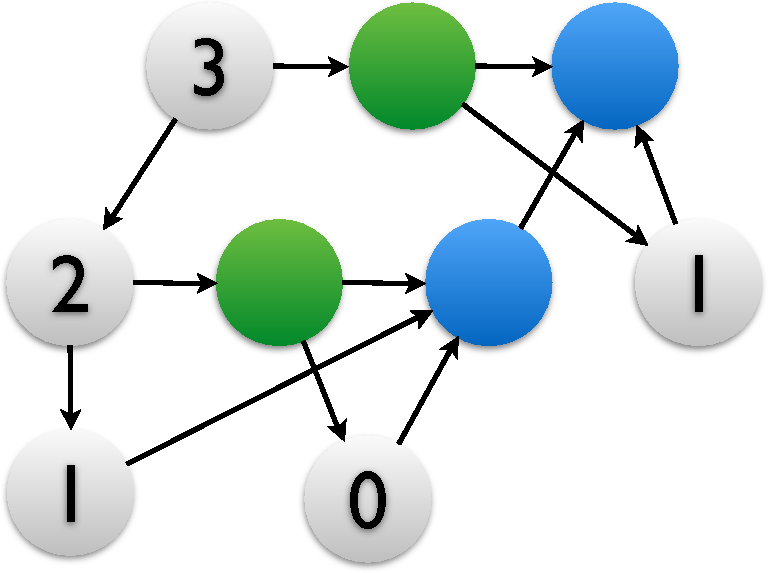
\includegraphics[width=\textwidth]{dag-strict-crop}
      \end{center}
    \end{column}
    %
    \begin{column}{0.5\textwidth}
      \begin{center}
	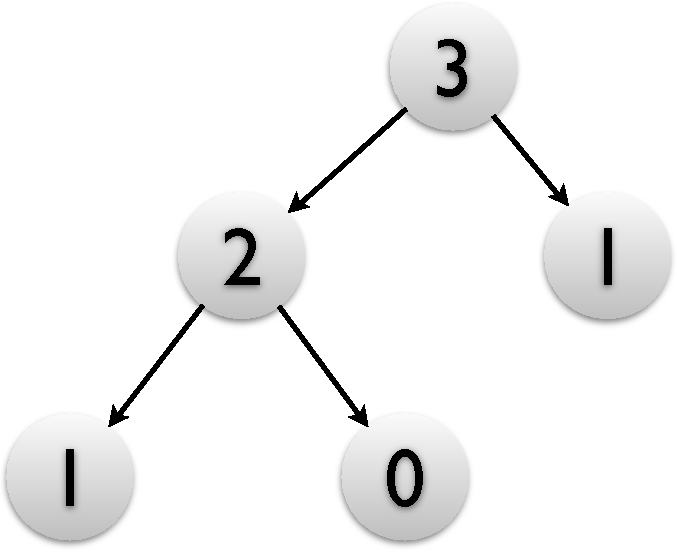
\includegraphics[width=\textwidth]{dag-dfg-crop}
      \end{center}
    \end{column}
  \end{columns}
\end{frame}
%------------------------------------------------------------------------------
\begin{frame}
  \frametitle{DAG of Fibonacci $n = 3$}
  \vspace{-10mm}
  \begin{center}
%    \hspace*{-6mm}
    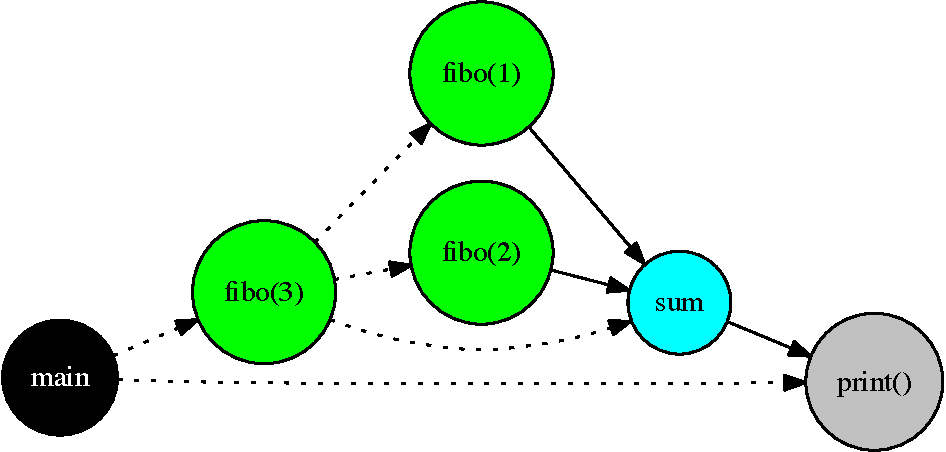
\includegraphics[width=\textwidth]{fibo/fibo4-clean-graph-crop}
  \end{center}
\end{frame}
%------------------------------------------------------------------------------
\begin{frame}
  \frametitle{DAG of Fibonacci $n = 3$}
  \vspace{-12mm}
  \begin{center}
    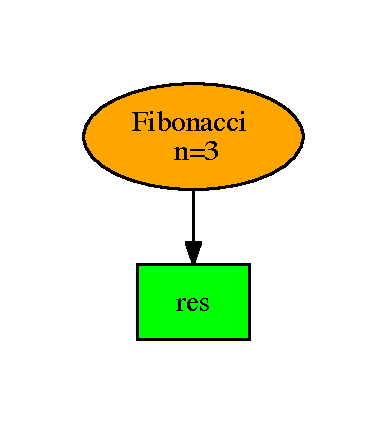
\includegraphics[scale=0.8]{fibo-graph-1}
  \end{center}
\end{frame}
%------------------------------------------------------------------------------
\begin{frame}
  \frametitle{DFG of Fibonacci $n = 3$}
  \vspace{-12mm}
  \begin{center}
    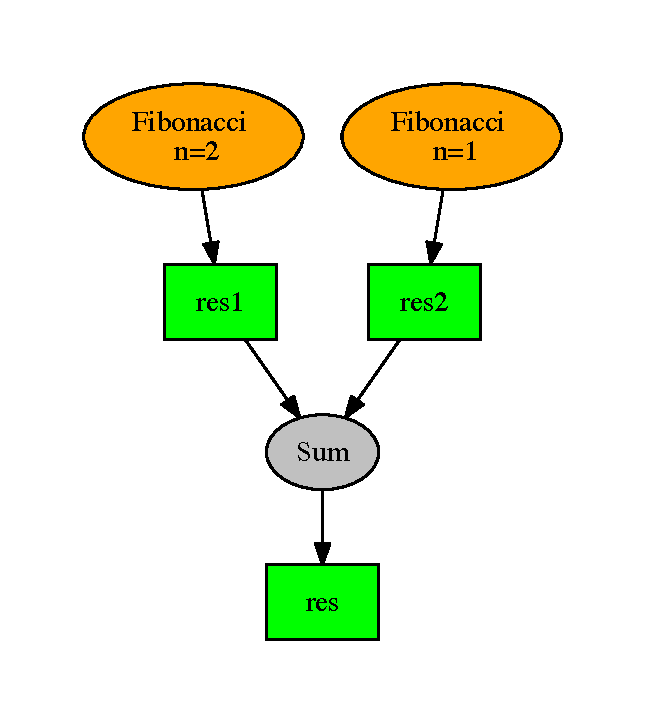
\includegraphics[scale=0.6]{fibo-graph-2}
  \end{center}
\end{frame}
%------------------------------------------------------------------------------
\begin{frame}
  \frametitle{DFG of Fibonacci $n = 3$}
  \vspace{-10mm}
  \begin{center}
    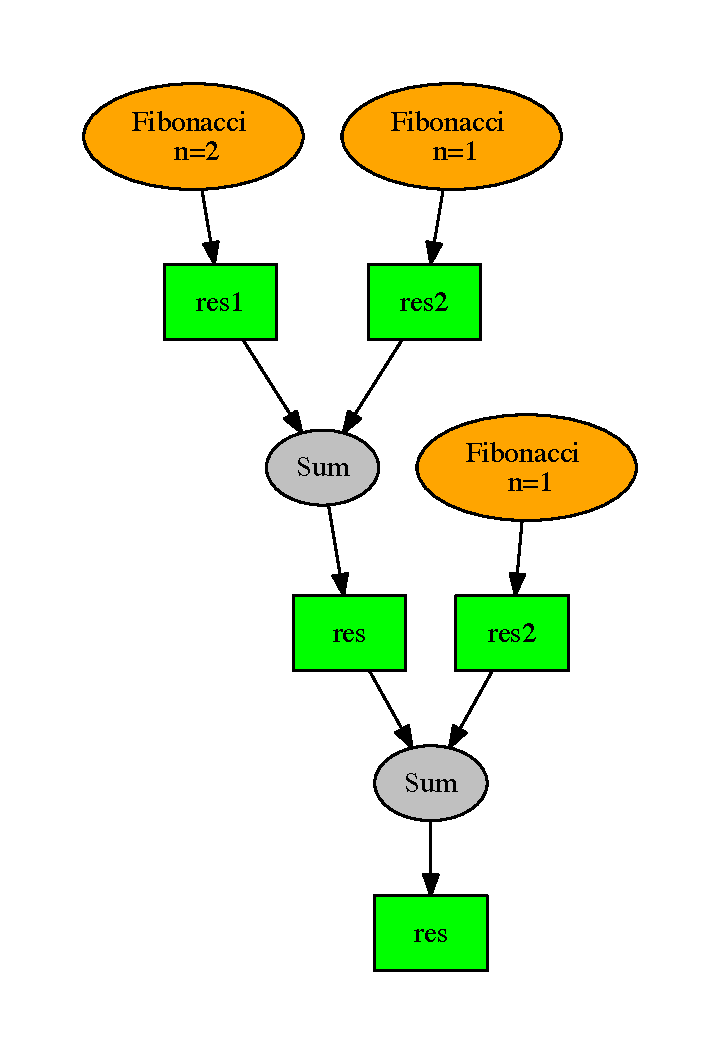
\includegraphics[scale=0.5]{fibo-graph-3}
  \end{center}
\end{frame}
%------------------------------------------------------------------------------
\begin{frame}
  \frametitle{DFG of Fibonacci $n = 3$}
  \vspace{-8mm}
  \begin{columns}
    \begin{column}{0.2\textwidth}
      \hspace*{-10mm}
      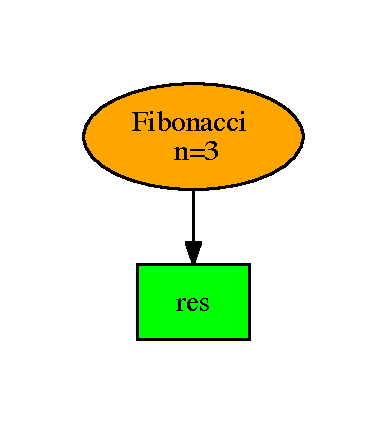
\includegraphics[scale=0.6]{fibo-graph-1}
    \end{column}
    %
    \begin{column}{0.4\textwidth}
      \hspace*{-10mm}
      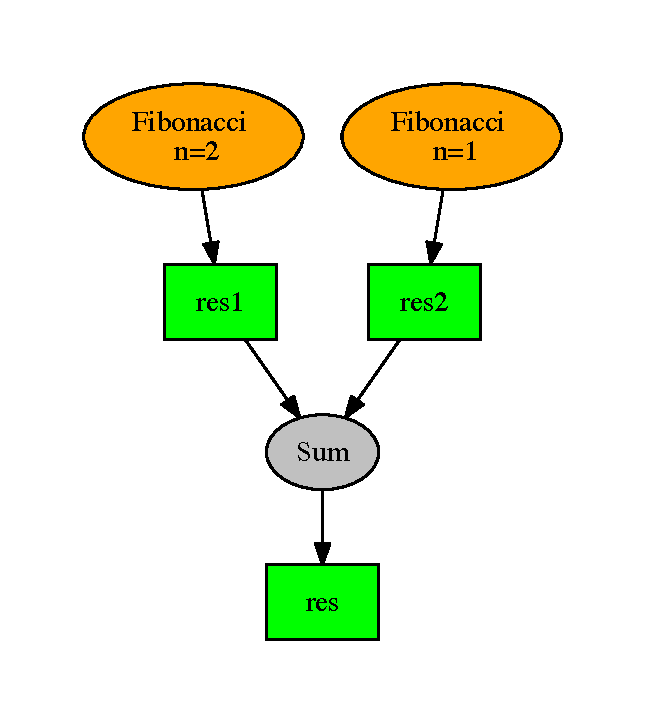
\includegraphics[scale=0.6]{fibo-graph-2}
    \end{column}
    %
    \begin{column}{0.4\textwidth}
      \hspace*{-10mm}
      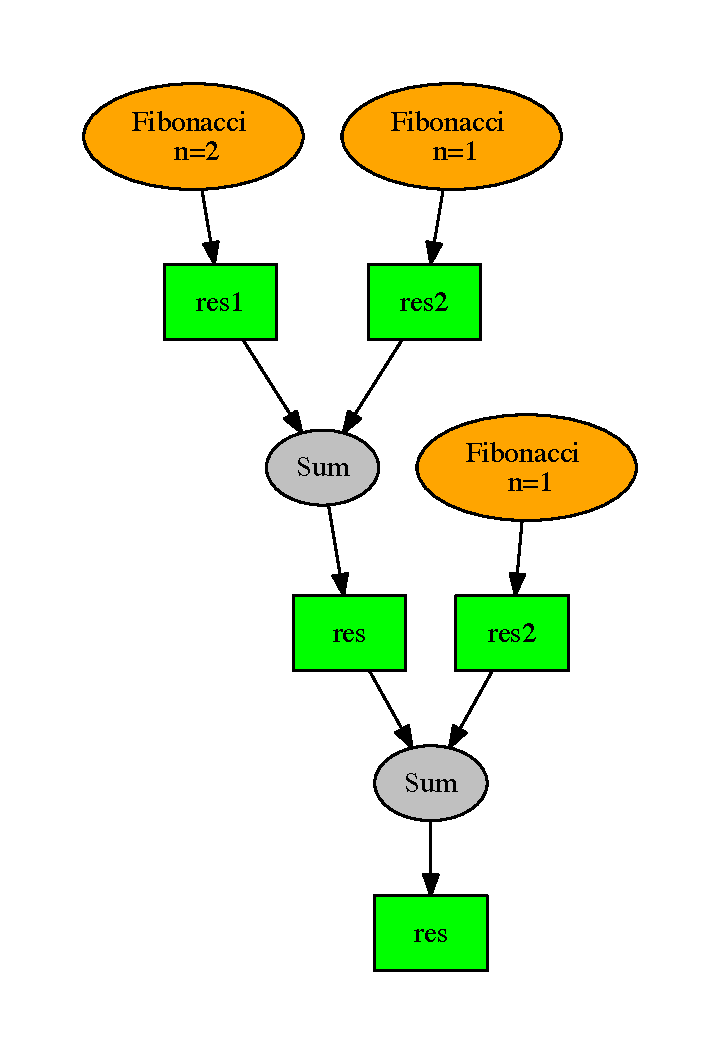
\includegraphics[scale=0.5]{fibo-graph-3}
    \end{column}
  \end{columns}
\end{frame}
%------------------------------------------------------------------------------
\begin{frame}
  \frametitle{DFG of Fibonacci $n = 3$}
  \vspace{-10mm}
  \begin{center}
%    \hspace*{-10mm}
    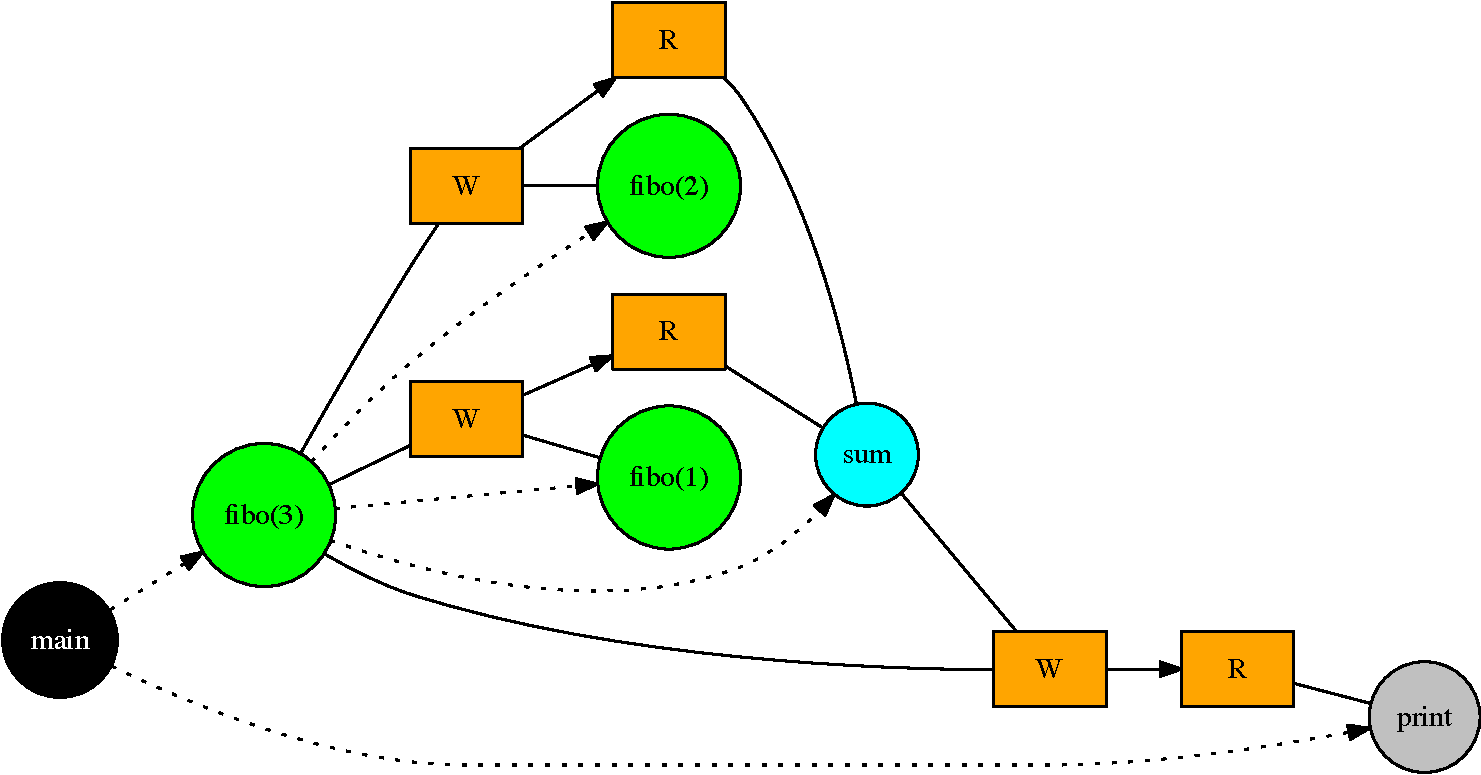
\includegraphics[width=\textwidth]{fibo/fibo4-graph-crop}
  \end{center}
\end{frame}
%------------------------------------------------------------------------------
\begin{frame}
  \frametitle{DFG of Fibonacci $n = 3$ (cumulative)}
  \vspace{-10mm}
  \begin{center}
%    \hspace*{-10mm}
    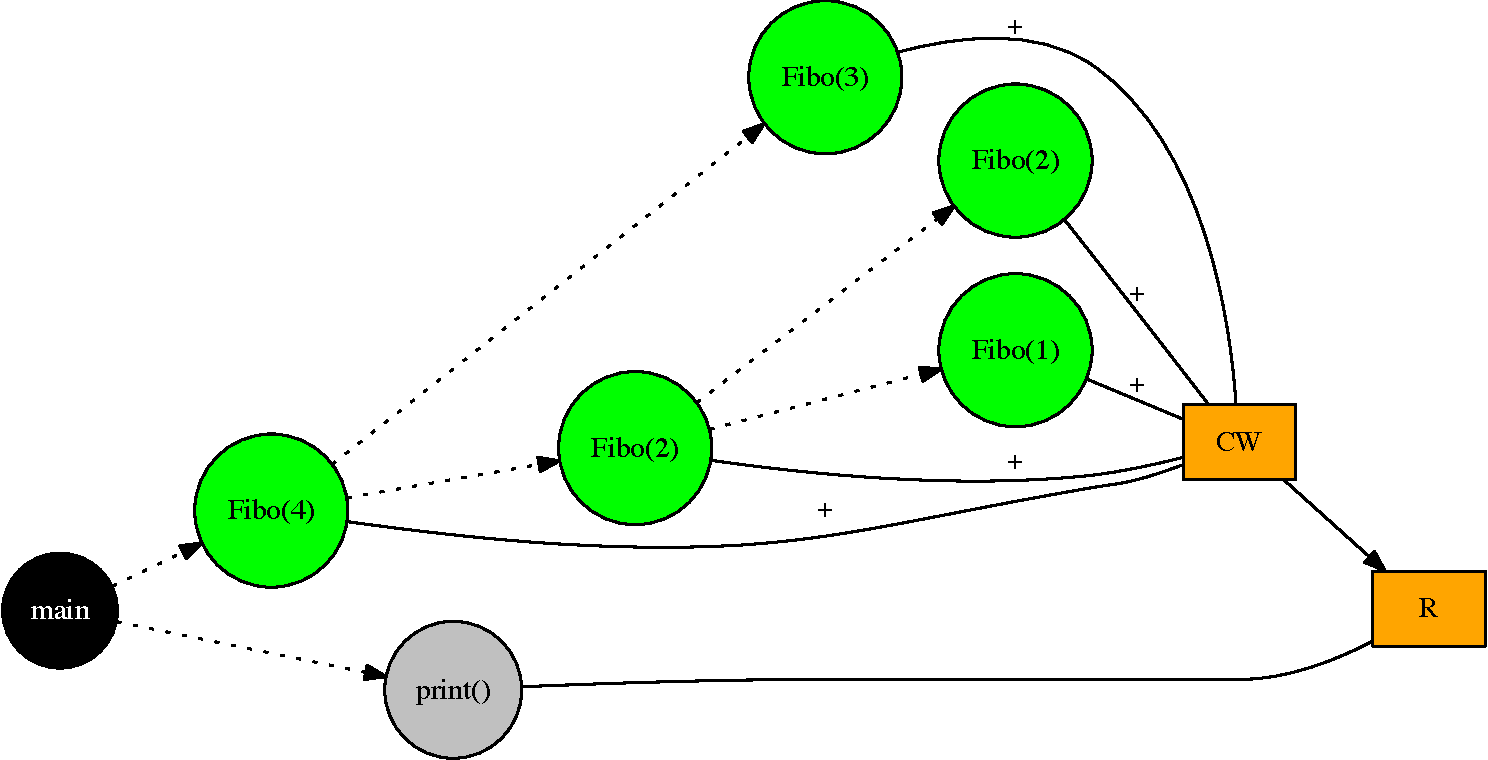
\includegraphics[width=\textwidth]{fibo/fibo4-cw-graph-crop}
  \end{center}
\end{frame}
%------------------------------------------------------------------------------
\begin{frame}
  \frametitle{DFG of Cholesky factorization}
  \vspace{-10mm}
  \begin{center}
%    \hspace*{-10mm}
    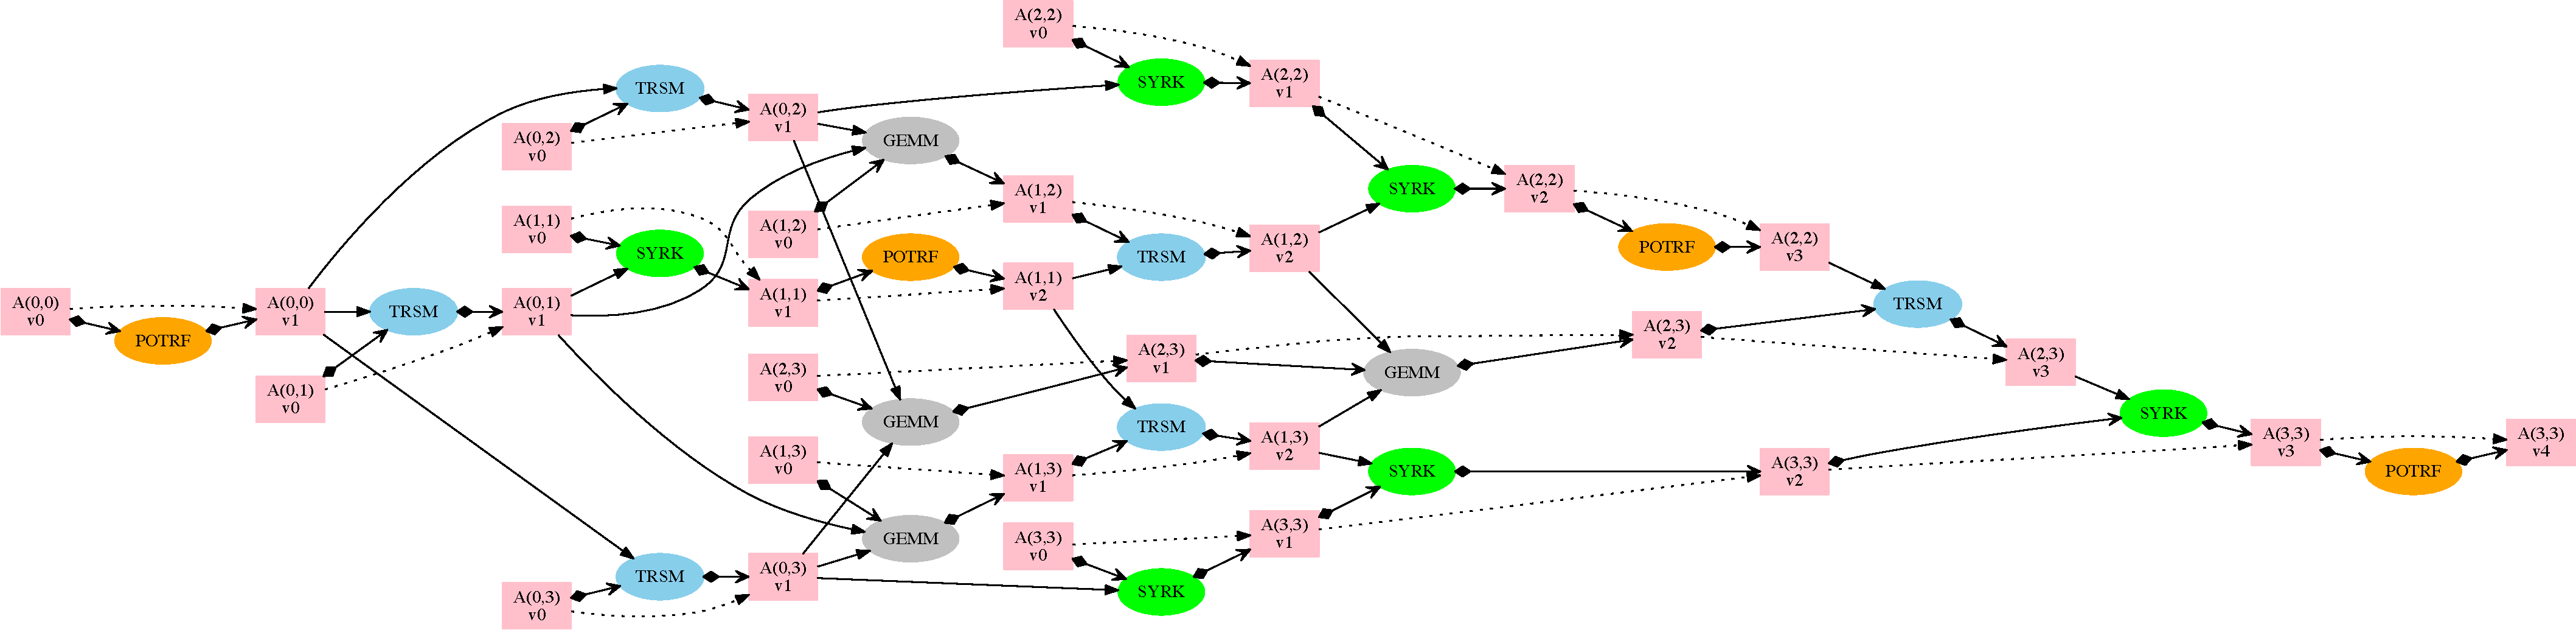
\includegraphics[width=\textwidth]{graph-cholesky-DFG-crop}
  \end{center}
\end{frame}
%------------------------------------------------------------------------------
\begin{frame}
  \frametitle{DFG of Cholesky factorization}
  \vspace{-2mm}
  \begin{center}
    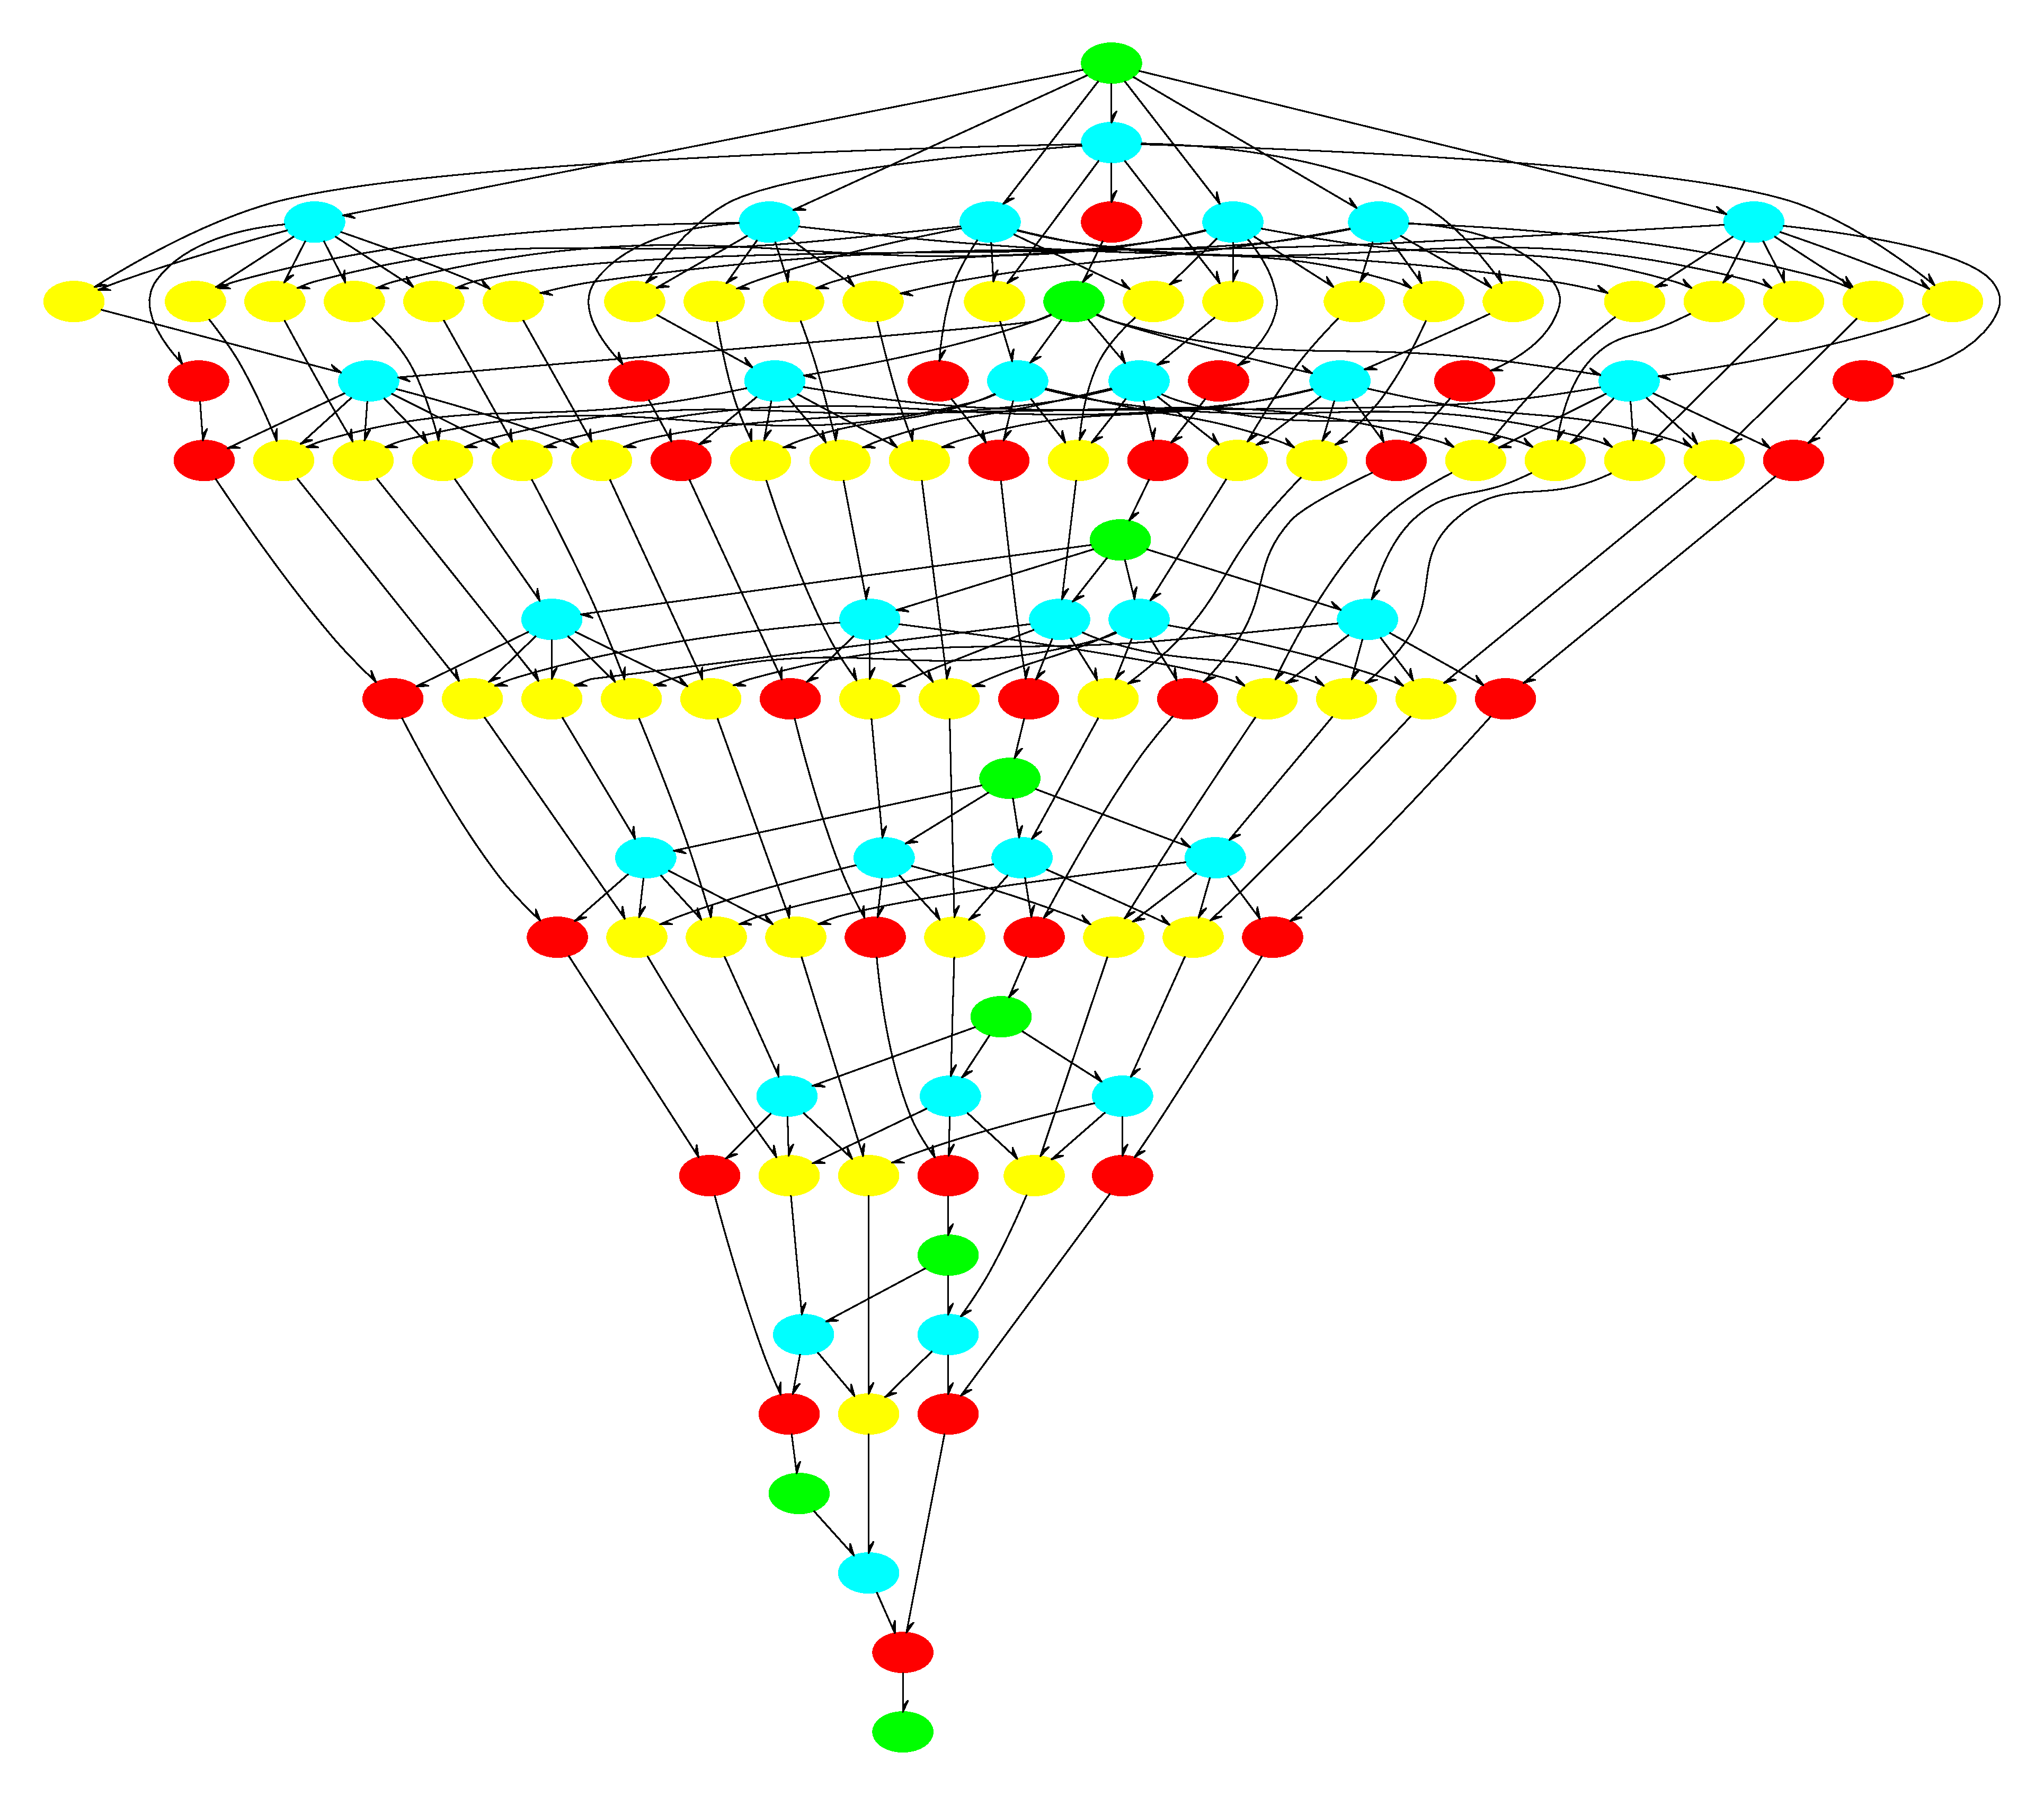
\includegraphics[width=0.8\textwidth]{cholesky}
  \end{center}
\end{frame}
%------------------------------------------------------------------------------
\begin{frame}
  \frametitle{DFG of Blocked matrix multiplication}
  \vspace{-10mm}
  \begin{center}
%    \hspace*{-10mm}
    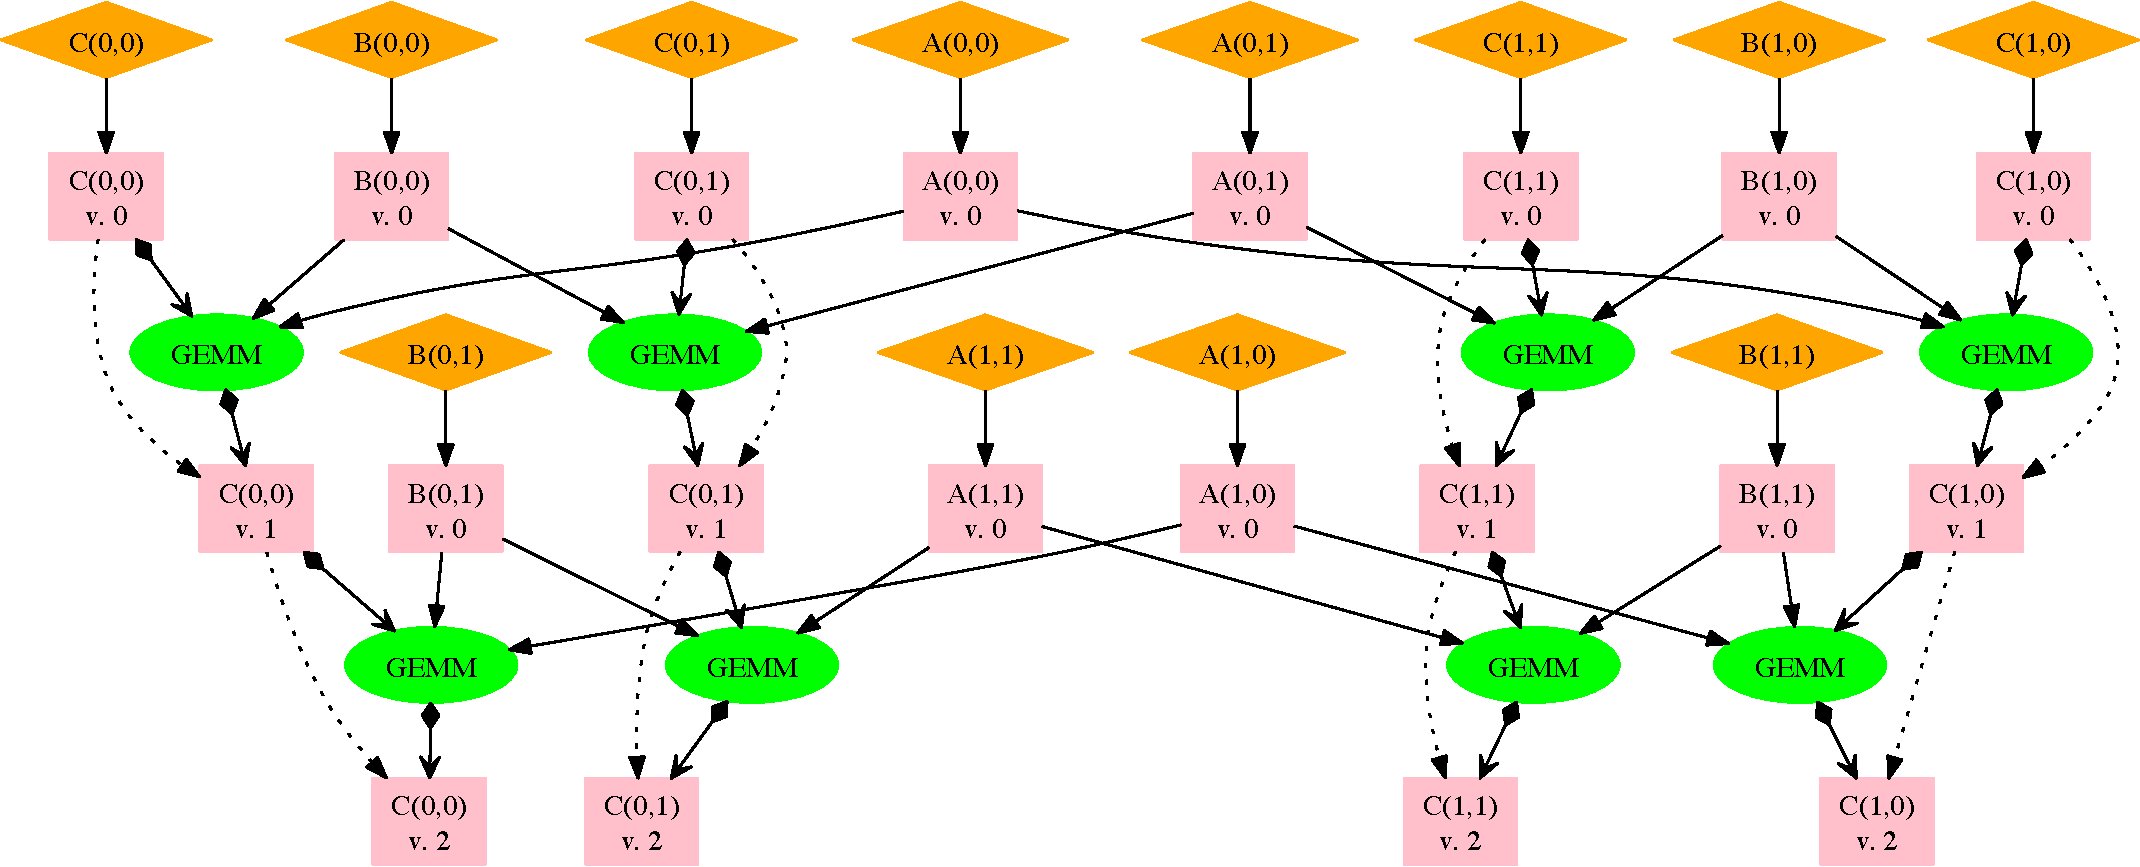
\includegraphics[width=\textwidth]{graph-gemm-DFG-crop}
  \end{center}
\end{frame}
%------------------------------------------------------------------------------

%%%%%%%%%%%%%%%%%%%%%%%%%%%%%%%%%%%%%%%%%%%%%%%%%%%%%%%%%%%%%%%%%%%%%%%%%%%%%%%%
\section{Programming interfaces}
%%%%%%%%%%%%%%%%%%%%%%%%%%%%%%%%%%%%%%%%%%%%%%%%%%%%%%%%%%%%%%%%%%%%%%%%%%%%%%%
%------------------------------------------------------------------------------
%%%%%%%%%%%%%%%%%%%%%%%%%%%%%%%%%%%%%%%%%%%%%%%%%%%%%%%%%%%%%%%%%%%%%%%%%%%%%%%
\subsection{OmpSs}
%------------------------------------------------------------------------------
\begin{frame}
  \frametitle{OmpSs}
  \begin{itemize}
  \item Task-based data flow programming model with single address space.
  \item Target platforms:
    \begin{itemize}
    \item multicore / SMP machines.
    \item heterogeneous systems (GPUs, Cell BE).
    \item clusters / distributed systems.
    \end{itemize}
  \item Based on OpenMP \blue{pragmas}.
    \begin{itemize}
    \item OpenMP + StarSs extensions.
    \end{itemize}
  \end{itemize}
  %
  \begin{block}{Data dependency}
    \begin{itemize}
    \item {\bf in} - read-only.
    \item {\bf out} - write-only.
    \item {\bf inout} - read and write.
    \item {\bf concurrent} - cumulative write.
    \end{itemize}
  \end{block}
\end{frame}
%------------------------------------------------------------------------------
\begin{frame}[fragile]
  \frametitle{OmpSs}
  %
  \begin{itemize}
  \item Task dependencies based on OpenMP.
  \end{itemize}
  %
  \begin{block}{}
\begin{lstlisting}
int main(void)
{
#pragma omp task out(result1)
  result1 = compute();

#pragma omp task in(result1)
  print(result1);

#pragma omp taskwait

  return 0;
}
\end{lstlisting}
  \end{block}
\end{frame}
%------------------------------------------------------------------------------
\begin{frame}[fragile]
  \frametitle{OmpSs}
  \begin{block}{}
\begin{lstlisting}
int reduce( int *a, int n ) {
  int i, result = 0;
  for(i= 0; i < n; i++){
#pragma omp task concurrent(result)
#pragma omp atomic
    result += a[i];
  }
  return result;
}

int main(void)
{
  int a[100];

#pragma omp task out(a)
  generate(a, 100);
  reduce(a, 100);

  return 0;
}
\end{lstlisting}
  \end{block}
\end{frame}
%------------------------------------------------------------------------------
\begin{frame}[fragile]
  \frametitle{Blocked matrix multiplication}
  \begin{block}{}
\begin{lstlisting}
#pragma omp target device (smp) 
#pragma omp task in([BS*BS]A, [BS*BS]B) inout([BS*BS]C)
void matmul_tile(float *A, float *B, float *C, int BS) {
  cblas_dgemm(CblasRowMajor, CblasNoTrans, CblasNoTrans,
       BS, BS, BS, 1.0, A, BS, B, BS, 1.0, C, BS);
}

void matmul(int mb, int nb, int kb,
                          float **A, float **B, float **C, int BS) { 
  int i, j, k;
  for(i = 0; i < mb; i++)
      for(j = 0; j < nb; j++)
        for(k = 0; k < kb; k++)
          matmul_tile(A[i*mb+k], B[k*kb+j], C[i*mb+j], BS);
}
\end{lstlisting}
\end{block}
\end{frame}
%------------------------------------------------------------------------------
\begin{frame}[fragile]
  \frametitle{OmpSs and GPUs}
  \begin{block}{}
\begin{lstlisting}
#pragma omp target device (smp) copy_deps
#pragma omp task 
void compute(void) {
    /* CPU */
}

#pragma omp target device (cuda) implements(compute) copy_deps
#pragma omp task 
void compute_cuda(void) {
    /* CUDA */
}

int main(void)
{
  compute();

  return 0;
}
\end{lstlisting}
  \end{block}
%
\pause
%
  \begin{alertblock}{Notice}
    In this tutorial, we do not detail heterogeneous systems.
  \end{alertblock}
\end{frame}
%------------------------------------------------------------------------------
\begin{frame}[fragile]
  \frametitle{Scheduling policy}
  \begin{itemize}
  \item {\bf breadth first} (\texttt{bf}) - global queue with tasks in FIFO.
  \item {\bf distributed breadth first} (\texttt{dbf}) - one queue per thread, with 
      task stealing.
  \item {\bf work first} (\texttt{wf}) - same of \texttt{dbf}, but it executes a 
    newly created task (depth-first).
  \item {\bf socket-aware} (\texttt{socket}) - per-socket level queue, it may use work stealing.
  \item {\bf versioning} (\texttt{versioning}) - multiple task implementations, using the 
    most suitable for the target.
  \end{itemize}
  %
  \begin{exampleblock}{Selecting a policy}
  \verb+$ NX_SCHEDULE=wf ./program+
  \end{exampleblock}
\end{frame}
%------------------------------------------------------------------------------
\begin{frame}[fragile]
  \frametitle{Installing OmpSs}
  \begin{itemize}
  \item Two step installation: \blue{Nanos++} and \blue{Mercurium C/++}.
    \begin{itemize}
    \item \blue{Nanos++}: runtime system.
    \item \blue{Mercurium C/C++ compiler}: compiler system (source-to-source).
    \end{itemize}
  \item Target \verb+export TARGET=$HOME/ompss+.
  \end{itemize}
  %
  \begin{block}{}
\begin{lstlisting}[language=]
$ cd ompss-yy.mm/nanox-version
$ ./configure --prefix=$TARGET
$ make
$ make install
\end{lstlisting}
  \end{block}
  %
  \begin{block}{}
\begin{lstlisting}[language=]
$ cd ompss-yy.mm/mcxx-version
$ ./configure --prefix=$TARGET --enable-ompss --with-nanox=$TARGET
$ make
$ make install
\end{lstlisting}
  \end{block}
  %
  \begin{alertblock}{Website}
    \begin{center}
      \url{https://pm.bsc.es/ompss}
    \end{center}
  \end{alertblock}
\end{frame}
%------------------------------------------------------------------------------
%%%%%%%%%%%%%%%%%%%%%%%%%%%%%%%%%%%%%%%%%%%%%%%%%%%%%%%%%%%%%%%%%%%%%%%%%%%%%%%
\subsection{StarPU}
%------------------------------------------------------------------------------
\begin{frame}
  \frametitle{StarPU}
  \begin{itemize}
  \item Runtime system for heterogeneous architectures.
    \begin{itemize}
    \item multi-CPUs, multi-GPUs, Cell BE.
    \end{itemize}

  \item Task-based programming model with data dependencies.

  \item Three main concepts:
    \begin{itemize}
    \item {\bf Codelet}  - describes a computational kernel.
    \item {\bf Task} - instance of a codelet.
    \item {\bf Data handle} - data entity that keeps track of copies over memory nodes.
    \end{itemize}
  \end{itemize}
\end{frame}
%------------------------------------------------------------------------------
%\begin{frame}[fragile]
%  \frametitle{StarPU vector scaling}
%  %
%  \begin{itemize}
%  \item First, select the \blue{performance model}.
%    \begin{itemize}
%    \item<2-> model type.
%    \item<3-> name of the 
%    \end{itemize}
%  \end{itemize}
%  %
%  \begin{block}{}
%\begin{lstlisting}[name=starpuvector,firstnumber=auto]
%/* Here it selects the history-based performance model */
%static struct starpu_perfmodel vector_scal_model = {
%  .type = STARPU_HISTORY_BASED,	
%  .symbol = "vector_scale_model"
%};
%
%\end{lstlisting}
%  \end{block}
%\end{frame}
%------------------------------------------------------------------------------
\begin{frame}[plain,fragile]
  \frametitle{StarPU vector scaling}
  %
  \begin{itemize}
  \item StarPU main program:
    \begin{itemize}
    \item<2-> Initialize StarPU with default configuration.
    \item<3-> Call the compute function.
    \item<4-> Terminate StarPU.
    \end{itemize}
  \end{itemize}
  %
  \begin{block}{}
\begin{lstlisting}[escapeinside={@}{@}]
int main(int argc, char **argv)
{
    float vector[NX];
    float factor = 3.14;
    
    @\alert<2>{starpu\_init(NULL);}@

    @\alert<3>{compute( vector, NX, factor );}@

    @\alert<4>{starpu\_shutdown();}@
    
    return 0;
}
\end{lstlisting}
  \end{block}
\end{frame}
%------------------------------------------------------------------------------
\begin{frame}[fragile]
  \frametitle{StarPU vector scaling}
  %
  \begin{itemize}
  \item Declaring a {\bf codelet}:
    \begin{itemize}
    \item<2-> Plug the kernel function.
    \item<3-> Declare the number of parameters used by the kernel.
    \item<4-> Declare the access mode of each parameter.
    \end{itemize}
  \end{itemize}
  %
  \begin{block}{}
\begin{lstlisting}[escapeinside={@}{@},name=starpuvector,firstnumber=auto]
static struct starpu_codelet cl = {
    @\alert<2>{.cpu\_funcs = \{vector\_scal\_cpu, NULL\},}@
    @\alert<3>{.nbuffers = 1,}@
    @\alert<4>{.modes = \{STARPU\_RW\}}@
};
\end{lstlisting}
  \end{block}
\end{frame}
%------------------------------------------------------------------------------
\begin{frame}[fragile]
  \frametitle{StarPU vector scaling}
  %
  \begin{itemize}
  \item Submitting a task:
    \begin{itemize}
    \item<2-> Tell StarPU to associate ``vector'' with a ``vector\_handle''.
    \item<3-> Insert a task in the StarPU DAG.
    \item<4-> Wait for tasks to complete.
    \item<5-> Stop data monitoring.
    \end{itemize}
  \end{itemize}
  %
  \begin{block}{}
\begin{lstlisting}[escapeinside={@}{@}]
void compute(float* vector, float factor, int n)
{
    @\alert<2>{starpu\_data\_handle\_t vector\_handle;}@
    @\alert<2>{starpu\_vector\_data\_register(\&vector\_handle, 0, (uintptr\_t)vector,}@
                                @\alert<2>{n, sizeof(vector[0]));}@

    @\alert<3>{ret = starpu\_insert\_task( \&cl,}@
                 @\alert<3>{STARPU\_VALUE, \&factor, sizeof(factor),}@
                 @\alert<3>{STARPU\_RW, vector\_handle,}@
                 @\alert<3>{0);}@

    @\alert<4>{starpu\_task\_wait\_for\_all();}@
    @\alert<5>{starpu\_data\_unregister(vector\_handle);}@
}
\end{lstlisting}
  \end{block}
\end{frame}
%------------------------------------------------------------------------------
\begin{frame}[plain,fragile]
  \frametitle{StarPU vector scaling}
  \begin{itemize}
  \item Writing the {\bf kernel function} for CPU:
    \begin{itemize}
    \item<2-> Extract the argument's value.
    \item<3-> Handle and length of the vector.
    \item<4-> Get a pointer to the local copy of the vector.
    \item<5-> Scale the vector.
    \end{itemize}
  \end{itemize}
  %
  \begin{block}{}
\begin{lstlisting}[escapeinside={@}{@}]
void vector_scal_cpu(void *buffers[], void *cl_arg)
{
  unsigned i;
  float factor;

  @\alert<2>{starpu\_codelet\_unpack\_args(cl\_arg, \&factor);}@
  @\alert<3>{struct starpu\_vector\_interface *vector = buffers[0];}@
  @\alert<3>{unsigned n = STARPU\_VECTOR\_GET\_NX(vector);}@
  @\alert<4>{float *val = (float *)STARPU\_VECTOR\_GET\_PTR(vector);}@
  @\alert<5>{for (i = 0; i < n; i++)}@
     @\alert<5>{val[i] *= factor;}@
}
\end{lstlisting}
  \end{block}
\end{frame}
%------------------------------------------------------------------------------
\begin{frame}[fragile]
  \frametitle{Data access mode}
  \begin{itemize}
  \item \textbf{STARPU\_R} - read-only mode.
  \item \textbf{STARPU\_W} - write-only mode.
  \item \textbf{STARPU\_RW} -  read and write mode.
  \item \textbf{STARPU\_SCRATCH} - temporary buffer, with no dependency constraint.
  \item \textbf{STARPU\_REDUX} - cumulative write with reduction.
  \end{itemize}
\end{frame}
%------------------------------------------------------------------------------
\begin{frame}[fragile]
  \frametitle{Performance model}
  \begin{itemize}
  \item Some scheduling policies estimate execution time in advance.
    \begin{itemize}
    \item Ex.: dm, dmda, heft.
    \end{itemize}
  
  \item Codelets give the \blue{performance model} specifying:
    \begin{itemize}
    \item Model name.
    \item Model type.
    \end{itemize}

  \item Available performance models:
    \begin{itemize}
    \item \textbf{STARPU\_HISTORY\_BASED} - measured at runtime. Records the
    average time for each input/output sizes.
    \item \textbf{STARPU\_REGRESSION\_BASED} - linear regression model over different data sizes
       ($\alpha*n^\beta$).
    \item \textbf{STARPU\_NL\_REGRESSION\_BASED} - non-linear regression model ($\alpha*n^\beta+\gamma$).
    \item \textbf{STARPU\_COMMON} - the application provides an estimation.
    \item \textbf{STARPU\_PER\_ARCH} - the application provides an estimation per architecture.
    \end{itemize}
  \end{itemize}
\end{frame}
%------------------------------------------------------------------------------
\begin{frame}[fragile]
  \frametitle{Performance model}
  \begin{itemize}
  \item History-based example.
  \end{itemize}
  \begin{block}{}
\begin{lstlisting}[escapeinside={@}{@}]
static struct starpu_perfmodel vector_scal_model = {
    .type = STARPU_HISTORY_BASED,
    .symbol = "vector_scal"
};

static struct starpu_codelet cl = {
    .cpu_funcs = {vector_scal_cpu, NULL},
    .nbuffers = 1,
    .modes = {STARPU_RW}
    @\alert<2->{.model = \&vector\_scal\_model,}
};
\end{lstlisting}
  \end{block}
\end{frame}
%------------------------------------------------------------------------------
\begin{frame}[fragile]
  \frametitle{Performance model}
  \begin{itemize}
  \item Common (provided by the user).
  \end{itemize}
  \begin{block}{}
\begin{lstlisting}[escapeinside={@}{@}]
double gemm_cost(struct starpu_task *task, unsigned nimpl) 
{
    uint32_t nxC, nyC, nxA;

    nxC = starpu_matrix_get_nx(task->descr[2].handle);
    nyC = starpu_matrix_get_ny(task->descr[2].handle);
    nxA = starpu_matrix_get_nx(task->descr[0].handle);
    double cost = ((double)nxC)*((double)nyC)*((double)nxA/1000.0f/4.11f);
  
    return cost;
}

static struct starpu_perfmodel starpu_sgemm_model_common =
{
    .cost_function = gemm_cost,
    .type = STARPU_COMMON,
};
\end{lstlisting}
  \end{block}
\end{frame}
%------------------------------------------------------------------------------
\begin{frame}[fragile]
  \frametitle{StarPU compiler extensions}
  \begin{itemize}
  \item StarPU GCC plugin.
  \end{itemize}
  \begin{block}{}
\begin{lstlisting}[basicstyle=\scriptsize\ttfamily,escapeinside={@}{@}]
static void vector_scal (unsigned int size, float vector[size], float factor)
  __attribute__ ((task));

/* The CPU implementation.  */
static void vector_scal (unsigned int size, float vector[size], float factor)
{
    unsigned int i;
    for (i = 0; i < size; i++)
        vector[i] *= factor;
}

int main(int argc, char **argv)
{
    float factor = 3.14;
    float vector[NX] __attribute__ ((heap_allocated, registered));
    
#pragma starpu initialize

      vector_scal (vector, NX, factor);

#pragma starpu wait
#pragma starpu acquire vector

#pragma starpu shutdown
    return 0;
}
\end{lstlisting}
  \end{block}
\end{frame}
%------------------------------------------------------------------------------
\begin{frame}[fragile]
  \frametitle{StarPU + MPI}
  \vspace{-4mm}
  \begin{block}{}
\begin{lstlisting}[basicstyle=\scriptsize\ttfamily,escapeinside={@}{@}]
float *tab;
starpu_data_handle_t tab_handle;
int main(int argc, char **argv)
{
    MPI_Init(NULL, NULL);
    MPI_Comm_rank(MPI_COMM_WORLD, &rank);
    MPI_Comm_size(MPI_COMM_WORLD, &size);

    @\alert<2->{starpu\_init}@(NULL);
    @\alert<2->{starpu\_mpi\_init}@(NULL, NULL, 0);

    /* */
    for (loop = 0; loop < nloops; loop++) {
       if ((loop % 2) == (rank%2)) {
           @\alert<2->{starpu\_mpi\_send}@(tab_handle, other_rank, loop, MPI_COMM_WORLD);
       } else {
           MPI_Status status;
           @\alert<2->{starpu\_mpi\_recv}@(tab_handle, other_rank, loop, MPI_COMM_WORLD, &status);
       }
     }

    @\alert<2->{starpu\_mpi\_shutdown}@();
    @\alert<2->{starpu\_shutdown}@();
    MPI_Finalize();
    return 0;
}
\end{lstlisting}
  \end{block}
\end{frame}
%------------------------------------------------------------------------------
\begin{frame}[fragile]
  \frametitle{Scheduling policy}
  \begin{itemize}
  \item Basic scheduling steps:
    \begin{enumerate}[<2->]
    \item The scheduler activate tasks (\texttt{push} operation) when they become ready.
      \begin{itemize}
      \item They are not waiting for some task or data dependencies.
      \end{itemize}
    \item Workers pull tasks (\texttt{pop} operation) from the scheduler.
      \begin{itemize}
      \item Centralized or distributed queue, depending on the policy.
      \end{itemize}
    \end{enumerate}

  \item<3-> Support different scheduling policies.
    \begin{itemize}
    \item<4-> {\bf eager} - centralized scheduling.
    \item<5-> {\bf prio} - centralized scheduling, one queue sorted by priority.
    \item<6-> {\bf ws} (\emph{work stealing}) - one queue per worker, with stealing of tasks.
    \item<7-> {\bf dm} (\emph{deque model}) - based on HEFT, it schedules tasks to
    minimize the finish time.
    \item<8-> {\bf dmda} (\emph{deque model data aware}) - similar to \texttt{dm}, but it takes into 
      account data transfer time. 
    \end{itemize}

  \item<9-> StarPU default policy: \textbf{eager}.
    \begin{itemize}
    \item \verb+export STARPU_SCHED=dmda+
    \end{itemize}
  \end{itemize}
\end{frame}
%------------------------------------------------------------------------------
\begin{frame}[fragile]
  \frametitle{Installing StarPU}
  \begin{itemize}
  \item Installing from Ubuntu or Debian packages:
  \end{itemize}
  %
  \begin{block}{}
\begin{lstlisting}[language=]
$ apt-cache search starpu
$ sudo apt-get install libstarpu-1.1 libstarpu-dev
\end{lstlisting}
  \end{block}
  %
  \begin{itemize}
  \item Building from source files:
  \end{itemize}
  \begin{block}{}
\begin{lstlisting}[language=]
$ mkdir build
$ cd build
$ ../configure --prefix=$HOME/install/starpu
$ make
$ make install
\end{lstlisting}
  \end{block}
  %
  \begin{alertblock}{Website}
    \begin{center}
    \url{http://runtime.bordeaux.inria.fr/StarPU/}
    \end{center}
  \end{alertblock}
\end{frame}
%------------------------------------------------------------------------------
%%%%%%%%%%%%%%%%%%%%%%%%%%%%%%%%%%%%%%%%%%%%%%%%%%%%%%%%%%%%%%%%%%%%%%%%%%%%%%%
\subsection{XKaapi}
%------------------------------------------------------------------------------
\begin{frame}
  \frametitle{XKaapi}
  \begin{block}{Goal}
    \begin{itemize}
    \item \textbf{Write once, run anywhere}.
    \item Simplify the development of parallel applications.
    \item Target multiple parallel architectures (multicore, GPUs, Intel Xeon Phi).
    \end{itemize}
  \end{block}
  %
  \vspace*{-2mm}
  %
  \begin{columns}
    \begin{column}{0.6\textwidth}
%      {\bf\blue{Two step solution}}:
      \begin{exampleblock}{Two step solution}
      \begin{itemize}
      \item<2-> {\bf Definition of a programming model}
	\begin{itemize}
	\item Task based.
	  \begin{itemize}
	  \item recursive tasks, adaptive tasks.
	  \end{itemize}
	\item Data flow dependencies.
	  \begin{itemize}
	  \item computed at runtime.
	  \end{itemize}
	\end{itemize}
      \item<3-> {\bf Automatic load balancing}
	\begin{itemize}
	\item Work stealing based algorithms.
	\item HEFT, cost models.
	\item Theoretical analysis of performance.
	\end{itemize}
      \end{itemize}
      \end{exampleblock}
    \end{column}
    %%
    \begin{column}{0.4\textwidth}
      \begin{center}
	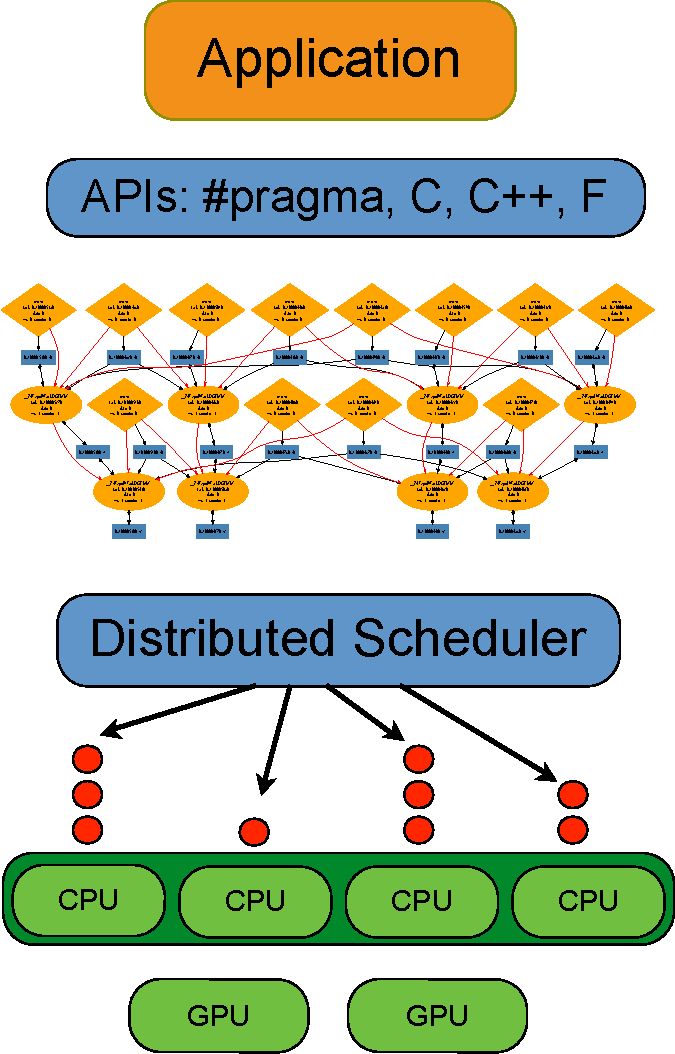
\includegraphics[width=0.7\textwidth]{kaapi-model-crop}
      \end{center}
    \end{column}
  \end{columns}
\end{frame}
%------------------------------------------------------------------------------
\begin{frame}[plain]
  \frametitle{XKaapi}
%  \vspace*{-5mm}
  \begin{figure}[ht]
  \centering
  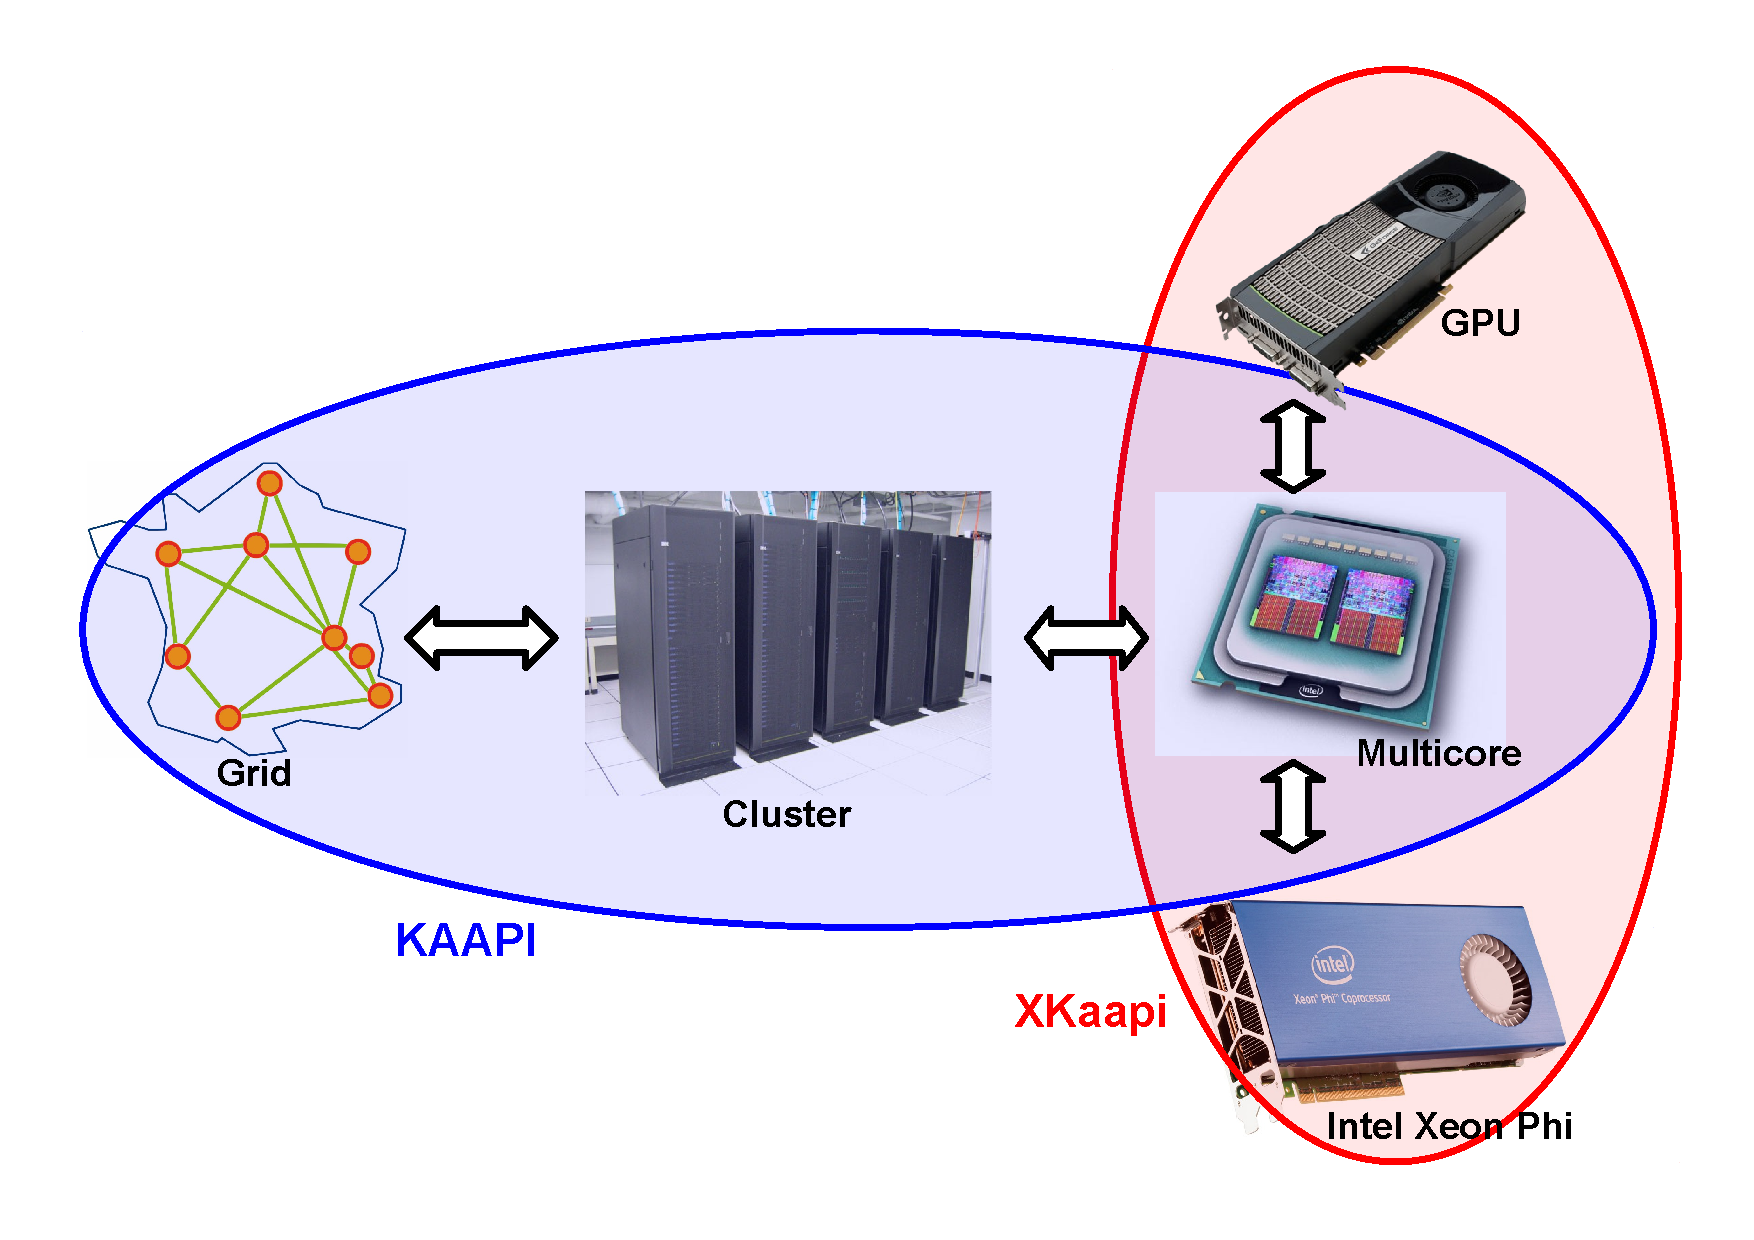
\includegraphics[width=\textwidth]{kaapi-vs-xkaapi}
  \end{figure}
\end{frame}
%------------------------------------------------------------------------------
\begin{frame}
  \frametitle{XKaapi design}
  \begin{itemize}
  \item \blue{Kernel}
    \begin{itemize}
    \item Runtime for APIs (or compiler).
    \item Work stealing internal scheduling.
    \item C language, fine grain implementation.
    \end{itemize}
  \end{itemize}

  \begin{itemize}
  \item \blue{APIs for different programming models}
    \begin{itemize}
    \item C++ API for multi-CPUs and multi-GPUs (CUDA).
    \item Two binary libraries (ABI) for OpenMP runtime
      \begin{itemize}
      \item libGOMP - GCC/OpenMP-3.1 + dependent tasks (4.0)
      \item libiomp5 - for ICC/OpenMP 3.1
      \end{itemize}
    \end{itemize}
  \end{itemize}
\end{frame}
%------------------------------------------------------------------------------
\begin{frame}[fragile]
  \frametitle{Kaapi++ API}
  \begin{itemize}
  \item Namespace \textbf{ka::}
  \end{itemize}
  %
  \begin{block}{Three main concepts}
    \begin{enumerate}
    \item {\bf Task signature} - declares parameters and their data access mode.
      \begin{itemize}
      \item Read (\verb+R+), Write (\verb+W+), Read Write (\verb+RW+),
	Cumulative Write (\verb+CW+).
      \end{itemize}
    \item {\bf Task implementation} - one implementation by architecture.
      \begin{itemize}
      \item Ex: CPU implementation, GPU implementation.
      \end{itemize}
    \item {\bf Shared data} - a data is shared between 2 tasks \textbf{iff}
      they have the same memory address in effective parameters.
    \end{enumerate}
  \end{block}
\end{frame}
%------------------------------------------------------------------------------
% \begin{frame}[fragile]
%   \frametitle{Kaapi++ API}
% \begin{block}{C++ function signature}
% \begin{lstlisting}
% void F( 
%     double n, 
%     double* result
% );
% \end{lstlisting}
% \end{block}
% %
% \pause
% %
% \begin{block}{\kaapixx task signature}
% \begin{lstlisting}
% struct TaskF: public ka::Task<2>::Signature<
%     double,       /* input parameter */
%     ka::W<double> /* output parameter */
% > {}; 
% \end{lstlisting}
% \end{block}
% \end{frame}
% %------------------------------------------------------------------------------
% \begin{frame}[fragile]
%   \frametitle{Kaapi++ API}
% \begin{block}{C++ function definition}
% \begin{lstlisting}
% void F ( 
%     double n, 
%     double* result
% ){
%     *result = n*n+1;
% }
% \end{lstlisting}
% \end{block}
% %
% \pause
% %
% \begin{block}{\kaapixx task body specialization}
% \begin{lstlisting}
% template<> struct TaskBodyCPU<TaskF> {
%     void operator() (
% 	double n,   
% 	ka::pointer_w<double> result
%     ){
% 	*result = n*n+1;
%     }
% };
% \end{lstlisting}
% \end{block}
% \end{frame}
% %------------------------------------------------------------------------------
\begin{frame}[fragile]
  \frametitle{Initialization}
%\hspace*{-4mm}
\begin{minipage}[t]{\textwidth}
%\vspace*{-6mm}
\begin{block}{}
\begin{lstlisting}
int main(int argc, char** argv) {
  try {
    /* Join the initial group of computation */
    ka::Community com = ka::System::join_community( argc, argv );
    
    /* Start computation by forking the main task */
    ka::SpawnMain<doit>()(argc, argv); 
    
    /* Leave the community */
    com.leave();

    /* */
    ka::System::terminate();
  }
  catch (const std::exception& E) {
    ka::logfile() << "Catch exception: " << E.what() << std::endl;
  }
  catch (...) {
    ka::logfile() << "Catch unknown exception: " << std::endl;
  }
  return 0;
}
\end{lstlisting}
\end{block}
\end{minipage}
\end{frame}
%------------------------------------------------------------------------------
\begin{frame}[fragile]
  \frametitle{Task entry point}
  \begin{itemize}
  \item Task ``\textbf{doit}'' spawned by the instruction \textbf{SpawnMain}.
  \end{itemize}
  %
  \begin{block}{}
  \begin{lstlisting}
/* Main task of the program
**/
struct doit {
  void operator()( int argc, char** argv )
  {
    double n = 3.1415;

    if( argc > 1 ) n = atof( argv[1] );

    /* ... */
  }
};
  \end{lstlisting}
  \end{block}
\end{frame}
%------------------------------------------------------------------------------
%\begin{frame}[fragile]
%  \frametitle{Kaapi++ tasks}
%  \begin{itemize}
%  \item {\bf Task signature}
%    \begin{itemize}
%    \item Define the number of parameters / type / access mode.
%    \end{itemize}
%  \end{itemize}
%  \vspace*{-4mm}
%\begin{block}{}
%\begin{lstlisting}
%/* Kaapi Hello task: print an integer n */
%struct TaskHello: public ka::Task<1>::Signature<int> {};
%\end{lstlisting}
%\end{block}
%%
%\pause
%%
%  \begin{itemize}
%  \item {\bf Task implementation}
%    \begin{itemize}
%    \item Specify an architecture implementation (CPU/GPU).
%    \end{itemize}
%  \end{itemize}
%  \vspace*{-4mm}
%\begin{block}{}
%\begin{lstlisting}
%/* CPU implementation */
%template<>
%struct TaskBodyCPU<TaskHello> {
%    void operator() ( int n )
%    {
%      std::cout << "Hello world in Kaapi!, n=" << n << std::endl;
%    }
%};
%\end{lstlisting}
%\end{block}
%\end{frame}
%------------------------------------------------------------------------------
\begin{frame}[fragile]
  \frametitle{Tasks}
  \begin{itemize}
  \item {\bf Task signature}
    \begin{itemize}
    \item Define the number of parameters / type / access mode.
    \end{itemize}
  \end{itemize}
  \vspace*{-4mm}
\begin{block}{}
\begin{lstlisting}
/* Kaapi Hello task: print a string and a double n */
struct TaskHello: public ka::Task<2>::Signature<std::string, double> {};
\end{lstlisting}
\end{block}
%
\pause
%
  \begin{itemize}
  \item {\bf Task implementation}
    \begin{itemize}
    \item Specify an architecture implementation (CPU/GPU).
    \end{itemize}
  \end{itemize}
  \vspace*{-4mm}
\begin{block}{}
\begin{lstlisting}
/* CPU implementation */
template<>
struct TaskBodyCPU<TaskHello> 
{
    void operator() ( std::string msg, double n )
    {
      std::cout << "Hello world in Kaapi!, msg=" << msg << ", n=" << n << std::endl;
    }
};
\end{lstlisting}
\end{block}
%
\begin{tikzpicture}[overlay,>=stealth]
\draw<3-> [draw=red,very thick] (5.8,6.1) circle (10pt);
\draw<3-> [draw=red,very thick] (9.1,6.1) ellipse (30pt and 12pt) node(a){};
\draw<3-> [draw=red,very thick] (10.8,6.1) circle (12pt) node(c){};
%
\draw<3-> [draw=red,very thick] (5.8,2.5) circle (12pt) node(b){};
\draw<3-> [draw=red,very thick] (7.8,2.5) circle (12pt) node(d){};
%
\draw<3-> [->,very thick,draw=red] (a) to (b) {};
\draw<3-> [->,very thick,draw=red] (c) to (d) {};
\end{tikzpicture}
\end{frame}
%------------------------------------------------------------------------------
\begin{frame}[fragile]
  \frametitle{Task creation}
  \begin{itemize}
  \item Keyword \textbf{spawn}.
  \end{itemize}
  \vspace*{-2mm}
\begin{block}{}
%\begin{lstlisting}
\begin{lstlisting}
/* Main task of the program */
struct doit {
  void operator()( int argc, char** argv )
  {
    double n = 3.1415;
    if( argc > 1 ) n = atof( argv[1] );

    ka::Spawn<TaskHello>()( "toto", n );
  }
};
\end{lstlisting}
\end{block}

\pause
%
  \begin{itemize}
  \item Write all arguments (integers).
  \end{itemize}
  \vspace*{-2mm}
\begin{block}{}
\begin{lstlisting}
/* The "doit" main task */
struct doit {
    void operator()( int argc, char** argv )
    {
      for(int i=1; i < argc; i++)
          ka::Spawn<TaskHello>()( std::string(argv[1]) );
    }
};
\end{lstlisting}
\end{block}
\end{frame}
%------------------------------------------------------------------------------
\begin{frame}[fragile]
  \frametitle{Execution order}
  \begin{itemize}
  \item Task creation is a non-blocking operation.
  \item the task (\blue{function call}) is pushed into a stack and the control flow
    continues without waiting for the termination. 
  \end{itemize}
  \vspace*{-2mm}
  \pause
\begin{block}{}
\begin{lstlisting}
/* The "doit" main task */
template<> struct doit {
    void operator()( int argc, char** argv )
    {
        int a;
        int* b;

        ka::Spawn<TaskThatRead_or_Write_Data>()( &a, &b );
    }
};
\end{lstlisting}
\end{block}
  \pause
  \begin{itemize}
  \item After the \blue{ka::Spawn}, task execution is not guarantee.
  \end{itemize}
\end{frame}
%------------------------------------------------------------------------------
\begin{frame}
  \frametitle{Execution order}
  \begin{itemize}
  \item Some guarantees:
    \begin{itemize}
    \item A task begins its execution when all its inputs are \red{produced}
      (\emph{data flow constraints}).
    \item  The parallel execution always produces the same result
      as the sequential execution.
    \item At the end, all created tasks have been executed. 
    \end{itemize}
  \item Notion of \blue{reference order} between tasks.
    \begin{itemize}
    \item Used to define execution order between any two tasks.
    \item Based on the Kaapi/XKaapi semantic (defined in Athapascan [1998]).
    \end{itemize}
  \end{itemize}
\end{frame}
%------------------------------------------------------------------------------
\begin{frame}[fragile]
  \frametitle{Execution order}
\begin{block}{Simple Hello world}
\begin{lstlisting}
/* The "doit" main task */
template<>
struct doit {
    void operator()( int argc, char** argv )
    {
      ka::Spawn<TaskHello>()( atoi(argv[1]) );
    }
};
\end{lstlisting}
\end{block}
%
\pause
%
\begin{block}{Possible outputs (two or mode cores)}
\begin{lstlisting}[language=]
> ./helloworld 1 2 
Hello World in Kaapi!, n=1
Hello World in Kaapi!, n=2

> ./helloworld 1 2 
Hello World in Kaapi!, n=2
Hello World in Kaapi!, n=1
\end{lstlisting}
\end{block}
\end{frame}
%------------------------------------------------------------------------------
\begin{frame}[fragile]
  \frametitle{How to enforce execution order}
  \begin{exampleblock}{Cilk's synchronization style}
    \begin{itemize}
    \item \verb+ka::Sync()+
    \item Force execution of all spawned tasks in the current task.
    \end{itemize}
  \end{exampleblock}
  %
  \pause
%  %
%  \begin{block}{Data flow constraint}
%    \begin{itemize}
%    \item \verb+ka::Sync( <pointer> )+
%    \item Wait until the pointed value is produced.
%    \end{itemize}
%  \end{block}
%  %
%  \pause
  %
  \begin{exampleblock}{Add dependencies between tasks}
    \begin{itemize}
    \item Describe \alert{access mode} of each task parameter.
    \end{itemize}
  \end{exampleblock}
\end{frame}
%------------------------------------------------------------------------------
\begin{frame}[fragile]
  \frametitle{Execution order}
\begin{block}{Simple Hello world (2 tasks)}
\begin{lstlisting}
/* The "doit" main task */
template<>
struct doit {
    void operator()( int argc, char** argv )
    {
      ka::Spawn<TaskHello>()( atoi(argv[1]) );
      ka::Sync();
      ka::Spawn<TaskHello>()( atoi(argv[1]) );
    }
};
\end{lstlisting}
\end{block}
%
\pause
%
\begin{block}{Possible outputs (two or mode cores)}
\begin{lstlisting}[language=]
> ./helloworld 1 2 
Hello World in Kaapi!, n=1
Hello World in Kaapi!, n=2

> ./helloworld 1 2 
Hello World in Kaapi!, n=1
Hello World in Kaapi!, n=2
\end{lstlisting}
\end{block}
%
\begin{tikzpicture}[overlay,>=stealth]
%\draw[<-] (1,1) .. (3,3) node[above] {\bf Cria};
\draw<3-> [<-,line width=2pt] (2.9,5.3) -- (9,5.3) node[shape=rectangle,fill=red!30] {Enforce order};
\draw<3-> [<-,line width=2pt] (4.6,2.2) -- (8,2.2) node[shape=rectangle,fill=green!30] {Always the same order};
%\node<3-> [shape=rectangle,fill=blue!20,below of=t1] {Recomendado quando $N = O(nthreads)$.};
\end{tikzpicture}
%
\end{frame}
%------------------------------------------------------------------------------
\begin{frame}[fragile]
  \frametitle{How to enforce execution order}
  \begin{itemize}
  \item Paramater rules: \blue{effective parameters}
    are mapped to \blue{formal parameters}.
  \end{itemize}
  %
  \pause
  %
  \begin{block}{By value}
    \begin{itemize}
    \item a copy is made into the task.
    \end{itemize}
  \end{block}
  %
  \pause
  %
  \begin{block}{By reference}
    \begin{itemize}
    \item No copy.
    \item But tasks must declare its acesses to shared data. 
    \item \textbf{read}: read access, the task can read the value.
    \item \textbf{write}: write access, a reader will see the written value.
    \item \textbf{read write}: exclusive access, one task has access to data.
    \item \textbf{cumulative write}:  several write will participate to produce the final
      value.
    \end{itemize}
  \end{block}
\end{frame}
%------------------------------------------------------------------------------
\begin{frame}[fragile]
  \frametitle{Task signature}
%\vspace*{-4mm}
%  \begin{itemize}
%  \item Número de parâmetros fixo em tempo de compilação.
%  \end{itemize}
%\hspace*{-4mm}
\begin{minipage}[t]{\textwidth}
\begin{block}{}
\begin{lstlisting}
/* Kaapi Hello task: print an integer n */
struct TaskFibo: public ka::Task<2>::Signature<ka::W<int>, int> {};
\end{lstlisting}
\end{block}
\end{minipage}
%
  \begin{itemize}
  \item<2-> \blue{Access mode}
    \begin{itemize}
    \item \verb+ka::W<T>+ - write.
    \item \verb+ka::R<T>+ - read.
    \item \verb+ka::RW<T>+ - read and write.
    \item \verb+ka::CW<T>+ - cumulative write with reduction.
    \end{itemize}
  \item<3-> \blue{Formal parameter}
    \begin{itemize}
    \item \verb+ka::pointer_w<T>+
    \item \verb+ka::pointer_r<T>+
    \item \verb+ka::pointer_rw<T>+
    \item \verb+ka::pointer_cw<T>+
    \end{itemize}
  \end{itemize}
\end{frame}
%------------------------------------------------------------------------------
\begin{frame}[fragile]
  \frametitle{Task implementation}
%  \vspace*{-4mm}
\begin{block}{}
\begin{lstlisting}
/* Kaapi Hello task: print an integer n */
struct TaskFibo: public ka::Task<2>::Signature<ka::W<long>, long> {};
\end{lstlisting}
\end{block}
%
\onslide<2->
%
\begin{block}{}
\begin{lstlisting}
/* CPU implementation */
template<>
struct TaskBodyCPU<TaskFibo> {
    void operator() ( ka::pointer_w<long> ptr, long n )
    {
        if (n < 2){ 
          *ptr = n; 
          return;
	} else {
          ka::auto_pointer<long> ptr1 = new long;
          ka::auto_pointer<long> ptr2 = new long;

          ka::Spawn<TaskFibo>() ( ptr1, n-1 );
          ka::Spawn<TaskFibo>() ( ptr2, n-2 );

          ka::Spawn<TaskSum>() ( ptr, ptr1, ptr2 );      
	}
    }
};
\end{lstlisting}
\end{block}
%
\begin{tikzpicture}[overlay,>=stealth]
\draw<3-> [draw=red,very thick] (5.7,7.8) circle (10pt);
\draw<3-> [draw=red,very thick] (9.3,7.8) circle (12pt) node(a){};
\draw<3-> [draw=red,very thick] (10.5,7.8) circle (12pt) node(c){};
%
\draw<3-> [draw=red,very thick] (6.2,5.8) circle (12pt) node(b){};
\draw<3-> [draw=red,very thick] (8.1,5.8) circle (12pt) node(d){};
%
\draw<3-> [->,very thick,draw=red] (a) to (b) {};
\draw<3-> [->,very thick,draw=red] (c) to (d) {};
\end{tikzpicture}
%
\end{frame}
%------------------------------------------------------------------------------
\begin{frame}
  \frametitle{Dependency}
  \begin{itemize}
  \item Task must describe its data access modes in effective parameters.
    \begin{itemize}
    \item Task signature.
    \item No side effect!
    \end{itemize}
  \item At runtime: execution $=$ sequence of tasks.
  \end{itemize}
  \begin{exampleblock}{XKaapi always respect the following dependencies:}
    \begin{itemize}
    \item A reader will see the value written by the last task in the reference order:
      \begin{itemize}
      \item W $\rightarrow$ R, {CW}* $\rightarrow$ R, ou RW $\rightarrow$ R: {\bf Read After Write}.
      \end{itemize}
    \item Other false dependencies (\textbf{Write after Read}) may be resolved by 
      \blue{additional data copies}.
      \begin{itemize}
      \item Runtime decision.
      \end{itemize}
    \end{itemize}
  \end{exampleblock}
\end{frame}
%------------------------------------------------------------------------------
\begin{frame}
  \frametitle{Dependency cost}
  \begin{block}{Dependency analysis is required to execute two tasks in parallel}
    \begin{itemize}
    \item Tasks with dependencies are executed following the \blue{reference order}.
      \begin{itemize}
      \item ``A reader will see the value written by the last writer''.
      \end{itemize}
    \item Tasks without dependencies may execute in parallel.
      \begin{itemize}
      \item The \blue{runtime} decides when and where 2 concurrent tasks will execute in parallel. 
      \end{itemize}
    \end{itemize}
  \end{block}
  %
  \pause
  %
  \begin{alertblock}{Work stealing scheduler}
    \begin{itemize}
    \item Execution following the reference order of execution.
      \begin{itemize}
      \item Only  \blue{dequeue}, no dependency analysis.
      \end{itemize}
    \item Dependencies are only computed during \blue{steal operation}.
    \end{itemize}
  \end{alertblock}
\end{frame}
%------------------------------------------------------------------------------
\begin{frame}[fragile]
  \frametitle{What is really shared ?}
  \begin{itemize}
  \item Two tasks sahred a common data \textbf{IFF} they access 
    the same data in memory.
  \item In the current implementation, it is a \red{limitation}.
    \begin{itemize}
    \item {\bf same data == same pointer}.
    \end{itemize}
  \end{itemize}
  %
\begin{block}{}
\begin{lstlisting}
ka::pointer<T> a;
ka::pointer<T> b = a + 100;
ka::Spawn<TaskRW1>()( a ); /* rw on a */
ka::Spawn<TaskRW2>()( b ); /* rw on b */
\end{lstlisting}
\end{block}
%
  \begin{alertblock}{No memory region (yet)}
  {\bf TaskRW1} and {\bf TaskRW2} are independent, even if 
  ``a'' and ``b'' overlap.
  \end{alertblock}
\end{frame}
%------------------------------------------------------------------------------
\begin{frame}[fragile]
  \frametitle{Example}
\begin{block}{}
\begin{lstlisting}[basicstyle=\scriptsize\ttfamily]
struct TaskFibo: public ka::Task<2>::Signature<ka::W<long>, long> {};

struct TaskDelete: public ka::Task<1>::Signature<ka::RW<long> > {};

struct TaskPrint: public ka::Task<1>::Signature<ka::R<long> > {};

int main( void ) {
  ka::pointer<long> res = new long;
  ka::Spawn<TaskFibo>()( res, n );


  ka::Spawn<TaskPrint>()( res );


  ka::Spawn<TaskDelete>()( res ); // free memory 
}
\end{lstlisting}
\end{block}
%
\begin{itemize}
\item The runtime automatically detects dependencies between tasks.
\item \blue{Write after Read} dependencies may be solved by copy.
\end{itemize}
%
\begin{tikzpicture}[overlay,>=stealth]
\draw<2-> [->,line width=2pt,red,bend left] (3.9, 4.1) .. controls(4.1,3.7) .. (3.9, 3.3) 
    node[above right=4pt,] {W $\rightarrow$ R (true) dependency};
\draw<2-> [->,line width=2pt,red,bend left] (3.9, 3.2) .. controls(4.1,2.8) .. (3.9, 2.4) 
    node[above right=4pt,] {R $\rightarrow$ RW (false) dependency};
\end{tikzpicture}
\end{frame}
%------------------------------------------------------------------------------
% \begin{frame}[fragile]
%   \frametitle{API Kaapi++}
% \begin{block}{C++ function calls}
% \begin{lstlisting}
% F(n, &result);
% Print(&result);
% \end{lstlisting}
% \end{block}
% %
% \pause
% %
% \begin{block}{\kaapixx task creation}
% \begin{lstlisting}
% ka::Spawn<TaskF>()(n, &result);
% ka::Spawn<TaskPrint>()(&result);
% ka::Sync();
% \end{lstlisting}
% \end{block}
% \end{frame}
%------------------------------------------------------------------------------
\begin{frame}[fragile]
  \frametitle{XKaapi source}
  \begin{itemize}
  \item \url{http://kaapi.gforge.inria.fr}
    \begin{itemize}
    \item Last version: \textbf{2.2}
    \end{itemize}
  \item Git: ligforge
    \begin{itemize}
    \item url $\rightarrow$ \url{ssh://git.ligforge.imag.fr/git/kaapi/xkaapi.git}
    \end{itemize}
  \item Git branches
    \begin{itemize}
    \item \verb+origin/master+: the oficial master branch.
    \item \verb+origin/<username>/<branch name>+: an user branch. 
    \end{itemize}
  \item Mailing list: \url{kaapi-leaders@lists.gforge.inria.fr}
    \begin{itemize}
    \item \url{http://lists.gforge.inria.fr/cgi-bin/mailman/listinfo/kaapi-leaders}
    \end{itemize}
  \end{itemize}
\end{frame}
%------------------------------------------------------------------------------
\begin{frame}[fragile]
  \frametitle{Installation}
  \begin{itemize}
  \item Requirement:
    \begin{itemize}
    \item GCC $>=$ 4.4 or Clang $>=$ 3.4
    \end{itemize}

  \item automake / autotools / etc...
    \begin{itemize}
    \item \verb+../xkaapi/configure --help+
    \item \verb+../xkaapi/configure --prefix=<prefixdir>+
    \item Usefull options:
      \begin{itemize}
      \item \verb+--enable-mode=release+ for performance.
      \item \verb+--enable-mode=debug+ for more assertions in the user level.
      \item \verb+--with-perfcounter+ for performance counter and tracing.
      \end{itemize}
    \end{itemize}
 
    \item Compiling \& installing
      \begin{itemize}
      \item make; make install
      \end{itemize}
  \end{itemize}
\end{frame}
%------------------------------------------------------------------------------
\begin{frame}[fragile]
  \frametitle{Running}
  \begin{itemize}
  \item \verb|KAAPI_CPUCOUNT=1 ./fibo_kaapi++ 30+|
      \begin{block}{}
      \begin{lstlisting}[language=]
Fibo(30)=832040
Time: 4.326541e-01
      \end{lstlisting}
      \end{block}
  \item \verb|KAAPI_CPUCOUNT=2 ./fibo_kaapi++ 30|
      \begin{block}{}
      \begin{lstlisting}[language=]
Fibo(30)=832040
Time: 2.143562e-01
      \end{lstlisting}
      \end{block}
  \item \verb|KAAPI_CPUSET=0:4,6 ./fibo_kaapi++ 30|
    \begin{itemize}
    \item Use cores 0,1,2,3,4 and 6 of the machine.
    \end{itemize}
  \end{itemize}
\end{frame}
%------------------------------------------------------------------------------
%------------------------------------------------------------------------------
% - %\subsection*{Installation de XKaapi}
% - \begin{frame}
% -   \frametitle{XKaapi installation}
% - 
% -   Installation (\p{make install}) into the directory \p{prefix}.
% - 
% -   Classic structure:
% -   \begin{itemize}
% -   \item \p{<prefix>/include} : header files
% -   \item \p{<prefix>/lib} : libraries
% -   \item \p{<prefix>/lib/pkgconfig} : \p{pkg-config} files
% -     to retrieve compilation flags 
% -   \item \p{<prefix>/share/doc/xkaapi} :  documentation
% -   \item \p{<prefix>/share/doc/xkaapi/examples} : examples in many APIs
% -     with a Makefile to compile
% -   \end{itemize}
% - \end{frame}
% - %------------------------------------------------------------------------------
% - %\subsection*{Installation alternative par paquets binaires}
% - %------------------------------------------------------------------------------
% - \begin{frame}
% -   \frametitle{Alternative installation}
% -   For Debian (Ubuntu ?), binary installation from packages.
% -   \begin{alertblock}{Attention}
% -     \begin{itemize}
% -     \item Packages are not in the official repositories.
% -     \item Compilation for the ``unstable'' distribution, see
% -       ``experimental'' (for CUDA 5)
% -     \end{itemize}
% -   \end{alertblock}
% - %
% -   \begin{enumerate}
% -   \item Add sources to \p{/etc/apt/sources.list}
% -     \begin{code}
% -       \hspace{-1cm}\footnotesize deb http://people.debian.org/~vdanjean/debian unstable main
% -     \end{code}
% -   \item \p{apt-get update}
% -   \item \p{apt-get install vdanjean-keyring}
% -   \item \p{apt-get update}
% -   \item \p{apt-get install libkaapi++-dev}
% -   \item \p{apt-get install -t experimental nvidia-cuda-toolkit libcupti-dev}
% -   \end{enumerate}
% - 
% - \end{frame}
% - %------------------------------------------------------------------------------
% - %\subsection{Compilation de programmes}
% - %------------------------------------------------------------------------------
% - \begin{frame}
% -   \frametitle{Compiling a XKaapi program}
% -   To compile a XKaapi program:
% -   \begin{enumerate}
% -   \item If the prefix is not standard (\p{/usr} ou \p{/usr/local}),
% -     configure \alert{\p{PKG\_CONFIG\_PATH}} :
% -     \begin{code}
% -       \footnotesize export PKG\_CONFIG\_PATH=<kaapi
% -       prefix>/lib/pkgconfig
% -     \end{code}
% - 
% -   \item Compile and link with \alert{\p{pkg-config}} :
% -     \begin{code}
% -       g++ -o mytest `pkg-config -{}-cflags kaapi++` $\backslash$ \\
% -       ~~~~`pkg-config -{}-libs kaapi++` mytest.cpp
% -     \end{code}
% -   \end{enumerate}
% - \end{frame}
% - %------------------------------------------------------------------------------
% - %\subsection{Exécution de programmes}
% - \begin{frame}
% -   \frametitle{Execute a XKaapi program}
% -   \begin{enumerate}
% -   \item If the prefix is not standard (\p{/usr} ou \p{/usr/local}),
% -     configure \alert{\p{LD\_LIBRARY\_PATH}} :
% -     \begin{code}
% -       \footnotesize export LD\_LIBRARY\_PATH=<kaapi prefix>/lib
% -     \end{code}
% - 
% -   \item Program execution:
% -     \begin{code}
% -       ./mytest
% -     \end{code}
% -   \end{enumerate}
% -   XKaapi can be ``configured'' with environment variables:
% -   \begin{code}\small
% -   \alert{KAAPI\_CPUCOUNT=1} ./fibo\_kaapi++ 30\\
% -   \structure{Fibo(30)=832040 Time: 4.326541e-01}\\
% -   \alert{KAAPI\_CPUCOUNT=2} ./fibo\_kaapi++ 30\\
% -   \structure{Fibo(30)=832040 Time: 2.143562e-01}\\
% -   \alert{KAAPI\_CPUSET=0:4,6} ./fibo\_kaapi++ 30\\
% -   \# use cores 0,1,2,3,4 and 6 of the machine
% -   \end{code}
% - 
% - \end{frame}
% - %------------------------------------------------------------------------------
% - %\subsection*{OpenMP et XKaapi}
% - \begin{frame}
% -   \frametitle{Execute an OpenMP program with XKaapi}
% -   \begin{enumerate}
% -   \item Compile the OpenMP program with \p{gcc} (with no XKaapi).
% -   \item Execute the program with the wrapper \p{libkomp-run}
% -     (installed into \p{<kaapi prefix>/bin}) :
% -     \begin{code}
% -       libkomp-run ./program-OpenMP
% -     \end{code}
% -   \item Compare execution against GCC runtime:
% -     \begin{code}
% -       ./program-OpenMP
% -     \end{code}
% -   \end{enumerate}
% - \end{frame}
% - %------------------------------------------------------------------------------
%%%%%%%%%%%%%%%%%%%%%%%%%%%%%%%%%%%%%%%%%%%%%%%%%%%%%%%%%%%%%%%%%%%%%%%%%%%%%%%
\subsection{OpenMP 4}
%------------------------------------------------------------------------------
%\begin{frame}
%  \frametitle{OpenMP 4}
%\end{frame}
%------------------------------------------------------------------------------
\begin{frame}[fragile]
  \frametitle{OpenMP 4}
  \begin{itemize}
  \item OpenMP 4.0 includes data dependency between tasks (\texttt{task}).
  \pause
  \item Directive \texttt{depend}
    \begin{itemize}
    \item \texttt{in} -- read.
    \item \texttt{out} -- write.
    \item \texttt{inout} -- read and write.
    \end{itemize}
  \pause
  \item Recursive synchronization by \texttt{taskgroup} construct.
    \begin{itemize}
    \item Synchronize a structured block.
    \item \texttt{taskgroup} waits for \alert{descendant tasks}.
    \item \texttt{taskwait} \alert{wait on the completion of child tasks}.
    \end{itemize}
  \end{itemize}
%
\pause
%
\begin{block}{Data flow dependency}
\begin{lstlisting}
#pragma omp taskgroup
{
  #pragma omp task depend(in:data) \
    depend(out:result)
  foo(data, result);
}
\end{lstlisting}
\end{block}
%
\end{frame}
%------------------------------------------------------------------------------
\begin{frame}[fragile]
  \frametitle{OpenMP 4}
\begin{block}{Fibonacci with OpenMP \texttt{depend}}
\begin{lstlisting}
int fib( int n ) {
  int x, y;
  if( n < 2 ) return n;
  #pragma omp taskgroup
  {
    #pragma omp task shared(x) depend(in:n) \
        depend(out:x)
    x = fib( n - 1);
    #pragma omp task shared(y) depend(in:n) \
      depend(out:y)
    y = fib( n - 2);
  }
  return x + y;
}
\end{lstlisting}
\end{block}
\end{frame}
%------------------------------------------------------------------------------
\begin{frame}[fragile]
  \frametitle{OpenMP 4 support}
  \begin{itemize}
  \item Clang with Intel OpenMP runtime library.
    \begin{itemize}
    \item \url{http://clang-omp.github.io/}
    \item \url{http://openmp.llvm.org/}
    \end{itemize}
  \item GCC (4.9) with libgomp runtime.
    \begin{itemize}
    \item \url{https://gcc.gnu.org/wiki/openmp}
    \end{itemize}
  \end{itemize}
\end{frame}
%------------------------------------------------------------------------------
%------------------------------------------------------------------------------

%%%%%%%%%%%%%%%%%%%%%%%%%%%%%%%%%%%%%%%%%%%%%%%%%%%%%%%%%%%%%%%%%%%%%%%%%%%%%%%%
\section{Data flow examples}
%%%%%%%%%%%%%%%%%%%%%%%%%%%%%%%%%%%%%%%%%%%%%%%%%%%%%%%%%%%%%%%%%%%%%%%%%%%%%%%
% %%%%%%%%%%%%%%%%%%%%%%%%%%%%%%%%%%%%%%%%%%%%%%%%%%%%%%%%%%%%%%%%%%%%%%%%%%%%%%%
% \subsection{Blocked matrix multiplication}
% %------------------------------------------------------------------------------
% \begin{frame}[plain,fragile]
%   \frametitle{Blocked matrix multiplication}
% \begin{block}{}
% \begin{lstlisting}[language=]
% for( i = 0; i < NB; i++ )
%     for( j = 0; j < NB; j++ )
%         for( k = 0; k < NB; k++ )
%             GEMM( A(i, k), A(k, j), A(i, j) );
% \end{lstlisting}
% \end{block}
% \end{frame}
% %------------------------------------------------------------------------------
% \begin{frame}[plain,fragile]
%   \frametitle{OmpSs}
% \begin{block}{}
% \begin{lstlisting}[basicstyle=\scriptsize\ttfamily]
% #pragma omp target device (smp) 
% #pragma omp task in([BS*BS]A, [BS*BS]B) inout([BS*BS]C)
% void matmul_tile(float *A, float *B, float *C, int BS) {
%   cblas_dgemm(CblasRowMajor, CblasNoTrans, CblasNoTrans,
%        BS, BS, BS, 1.0, A, BS, B, BS, 1.0, C, BS);
% }
% 
% void matmul(int mb, int nb, int kb,
%                           float **A, float **B, float **C, int BS) { 
%   int i, j, k;
%   for(i = 0; i < mb; i++)
%       for(j = 0; j < nb; j++)
%         for(k = 0; k < kb; k++)
%           matmul_tile(A[i*mb+k], B[k*kb+j], C[i*mb+j], BS);
% }
% \end{lstlisting}
% \end{block}
% \end{frame}
% %------------------------------------------------------------------------------
% \begin{frame}[plain,fragile]
%   \frametitle{StarPU}
% \begin{block}{}
% \begin{lstlisting}[basicstyle=\scriptsize\ttfamily]
% \end{lstlisting}
% \end{block}
% \end{frame}
% %------------------------------------------------------------------------------
% \begin{frame}[plain,fragile]
%   \frametitle{XKaapi}
% \begin{block}{}
% \begin{lstlisting}[basicstyle=\scriptsize\ttfamily]
% \end{lstlisting}
% \end{block}
% \end{frame}
% %------------------------------------------------------------------------------
%%%%%%%%%%%%%%%%%%%%%%%%%%%%%%%%%%%%%%%%%%%%%%%%%%%%%%%%%%%%%%%%%%%%%%%%%%%%%%%
\subsection{Tiled Cholesky factorization}
%------------------------------------------------------------------------------
\begin{frame}[plain,fragile]
  \frametitle{Tiled Cholesky factorization}
  \begin{itemize}
  \item Parallel algorithm from PLASMA [UTK].
  \end{itemize}
\begin{block}{}
\begin{lstlisting}[language=]
for( k = 0; k < NB; k++ ) {
    POTRF( A(k, k) );
    
    for( m = k+1; m < NB; m++ ){
        TRSM( A(k, k), A(m, k) );
    }

    for( m = k+1; m < NB; m++ ){
        SYRK( A(m, k), A(m, m) );

        for( n = k+1; n < m; n++ ){
           GEMM( A(m, k), A(n, k), A(m, n) );
	}
    }
}
\end{lstlisting}
\end{block}
\end{frame}
%------------------------------------------------------------------------------
\begin{frame}[plain,fragile]
  \frametitle{XKaapi}
  \vspace{-4mm}
  %
  \begin{block}{}
\begin{lstlisting}[basicstyle=\scriptsize\ttfamily]
struct TaskPOTRF: public ka::Task<3>::Signature
<
  CBLAS_ORDER,			      /* row / col */
  CBLAS_UPLO,             /* upper / lower */
  ka::RW<ka::range2d<double> > /* A */
>{};

struct TaskGEMM: public ka::Task<8>::Signature
<
  CBLAS_ORDER,			      /* row / col */
  CBLAS_TRANSPOSE,        /* NoTrans/Trans for A */
  CBLAS_TRANSPOSE,        /* NoTrans/Trans for B */
  double,                      /* alpha */
  ka::R<ka::range2d<double> >, /* Aik   */
  ka::R<ka::range2d<double> >, /* Akj   */
  double,                      /* beta */
  ka::RW<ka::range2d<double> > /* Aij   */
>{};
\end{lstlisting}
  \end{block}
\end{frame}
%------------------------------------------------------------------------------
\begin{frame}[plain,fragile]
  \frametitle{XKaapi}
  \vspace{-4mm}
\begin{block}{}
\begin{lstlisting}[basicstyle=\scriptsize\ttfamily]
struct TaskCholesky: public ka::Task<2>::Signature< ka::RPWP<ka::range2d<double> >, CBLAS_UPLO >{};

template<> struct TaskBodyCPU<TaskCholesky> {
  void operator()( ka::range2d_rpwp<double> A, const CBLAS_UPLO uplo)
  {
    size_t N = A->dim(0);
    size_t blocsize = global_blocsize;
    
    for (size_t k=0; k < N; k += blocsize) {
      ka::rangeindex rk(k, k+blocsize);
      ka::Spawn<TaskPOTRF>() ( A(rk,rk) );
      
      for (size_t m=k+blocsize; m < N; m += blocsize) {
        ka::rangeindex rm(m, m+blocsize);
        ka::Spawn<TaskTRSM>() (  A(rk,rk), A(rk,rm) );
      }
      
      for (size_t m=k+blocsize; m < N; m += blocsize) {
        ka::rangeindex rm(m, m+blocsize);
        ka::Spawn<TaskSYRK>() ( A(rk,rm), A(rm,rm) );
	
        for (size_t n=k+blocsize; n < m; n += blocsize) {
          ka::rangeindex rn(n, n+blocsize);
          ka::Spawn<TaskGEMM>() (  A(rk,rm), A(rk,rn), A(rn,rm) );
        }
      }
    }
  }
};
\end{lstlisting}
\end{block}
\end{frame}
%------------------------------------------------------------------------------
%\begin{frame}[plain,fragile]
%  \frametitle{XKaapi}
%\begin{block}{}
%\begin{lstlisting}[basicstyle=\scriptsize\ttfamily]
%\end{lstlisting}
%\end{block}
%\end{frame}
%------------------------------------------------------------------------------
\begin{frame}[plain]
  \frametitle{XKaapi data flow graph}
  \vspace*{-5mm}
  \begin{figure}[ht]
  \centering
  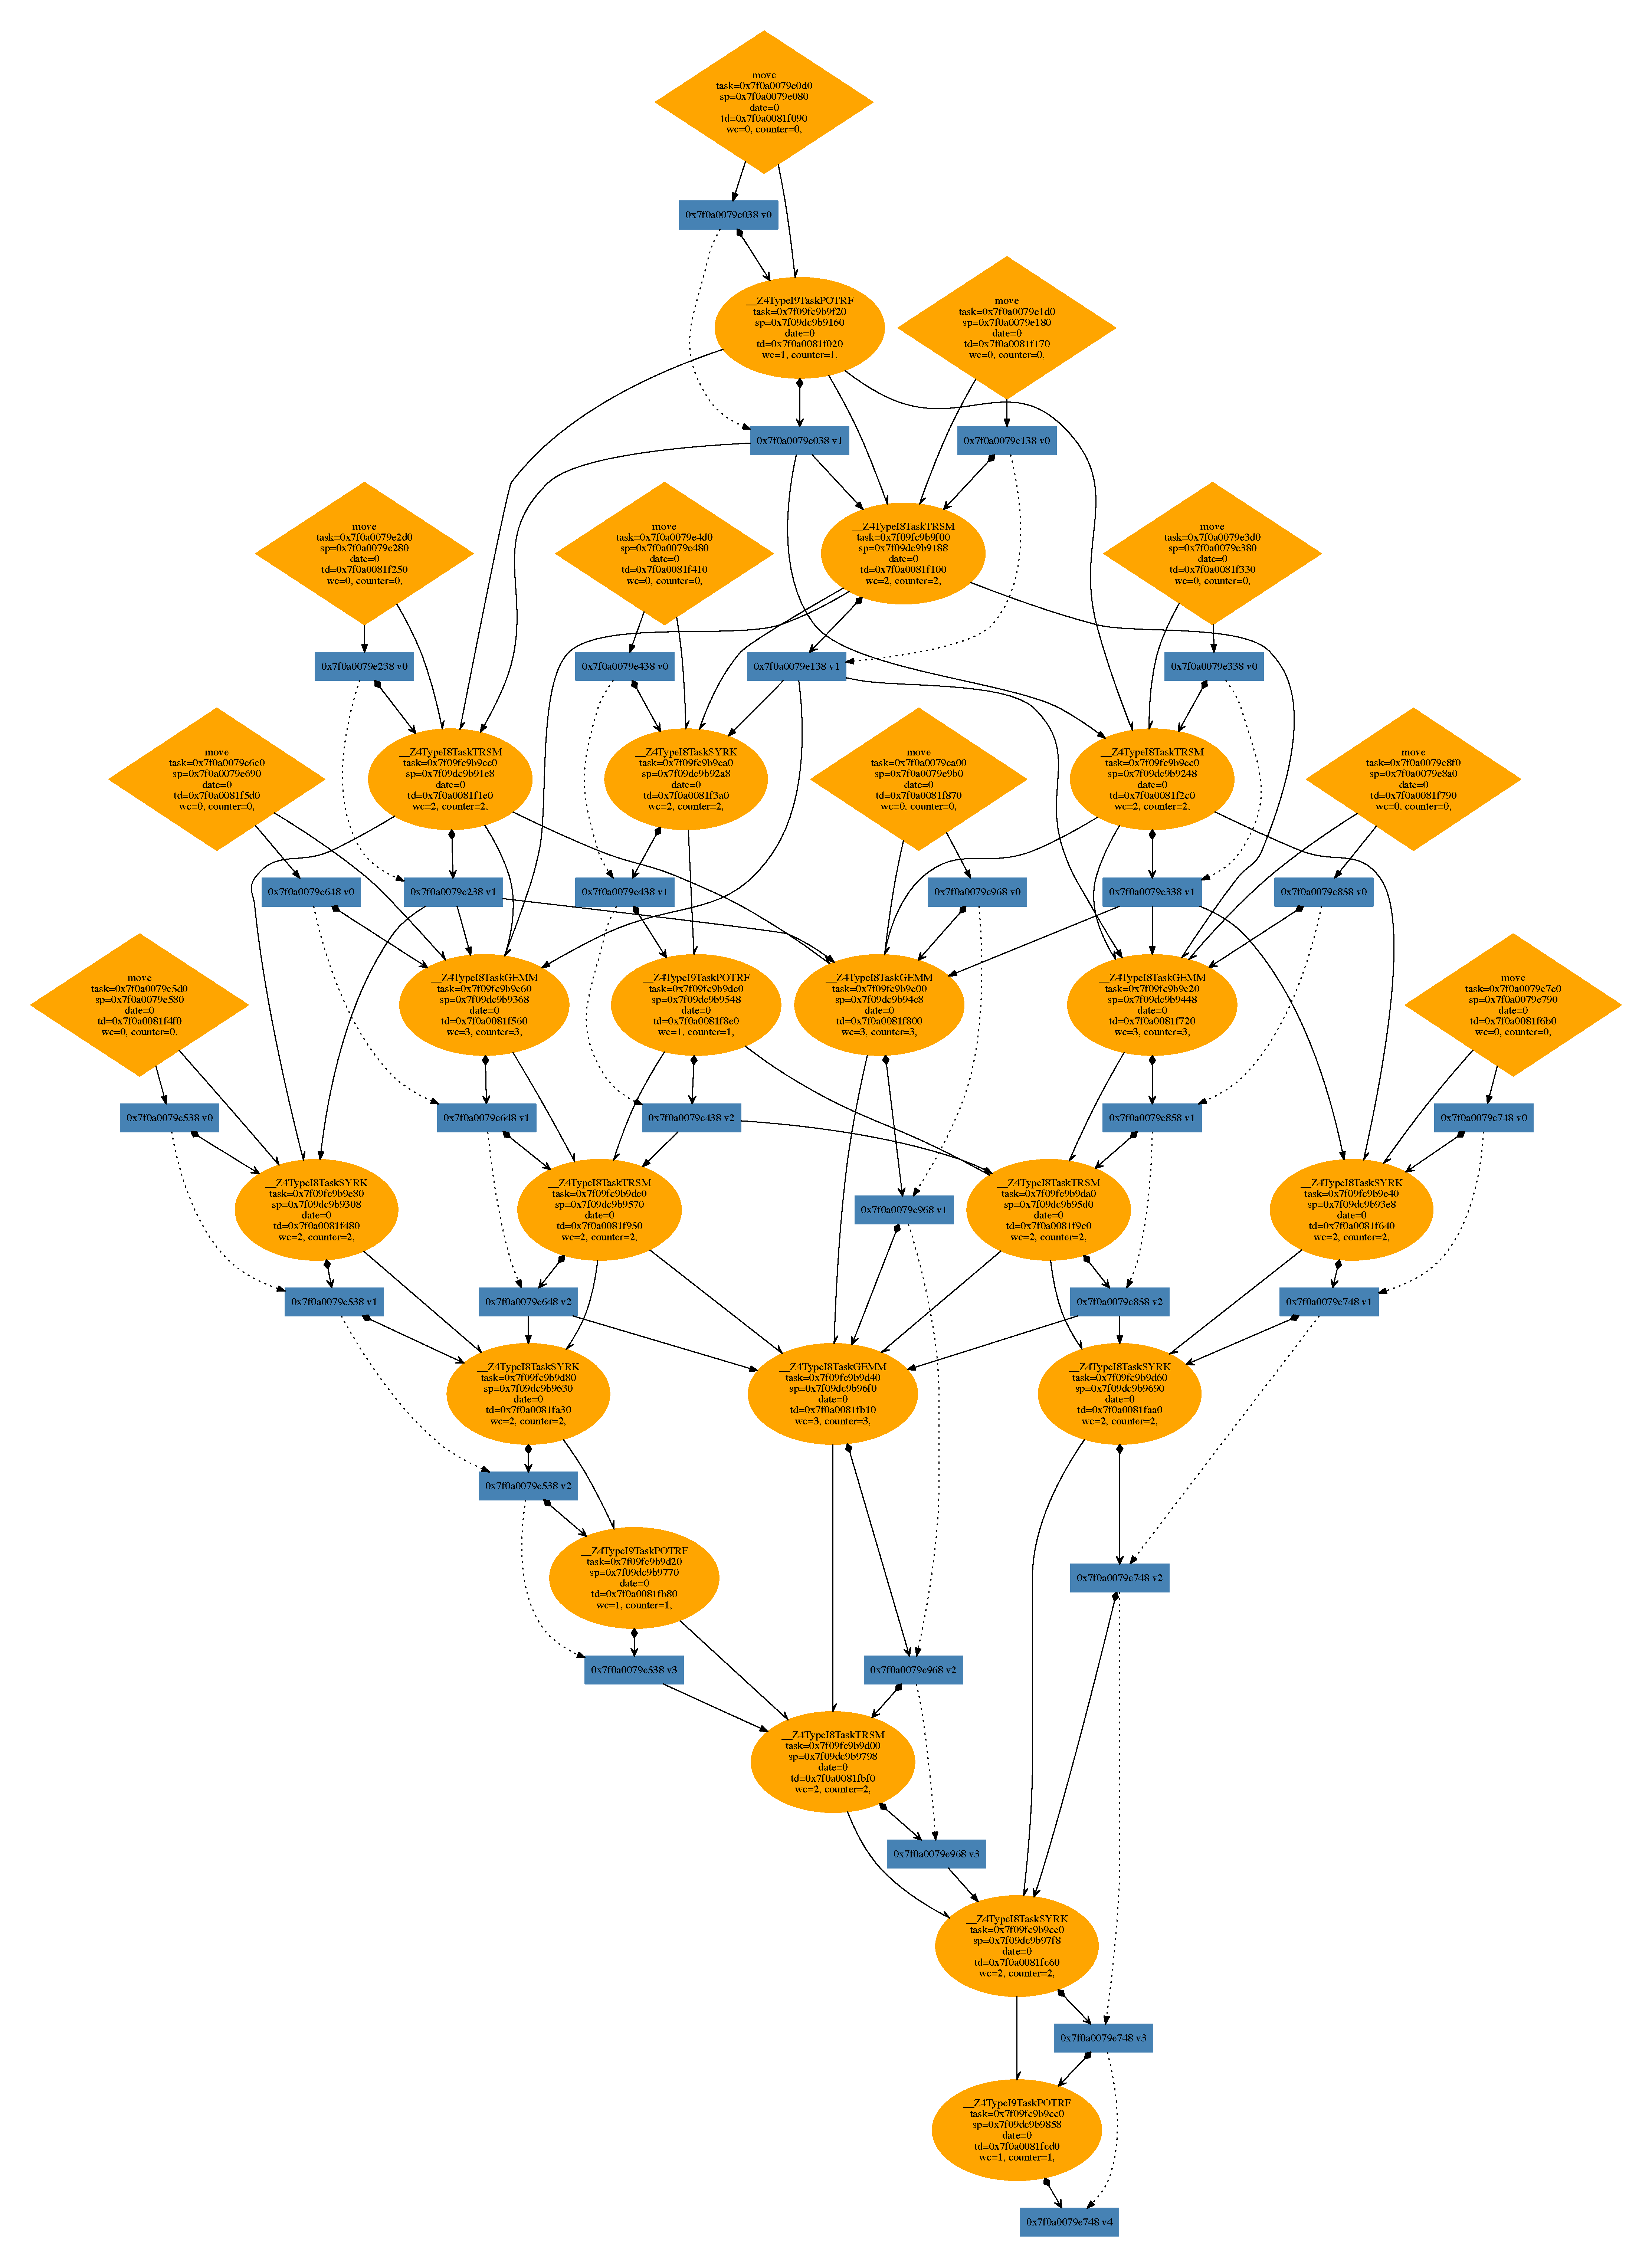
\includegraphics[width=0.5\textwidth]{chol-4096-1024}
  \end{figure}
\end{frame}
%------------------------------------------------------------------------------
\begin{frame}[plain,fragile]
  \frametitle{StarPU}
  \vspace{-4mm}
  %
  \begin{block}{}
\begin{lstlisting}[basicstyle=\scriptsize\ttfamily]
static struct starpu_codelet cl_dpotrf = {
    .modes = { STARPU_RW },
    .type = STARPU_SEQ,
    .where = STARPU_CPU,
    .cpu_funcs = {chol_cpu_codelet_update_dpotrf, NULL},
    .nbuffers = 1
};

static struct starpu_codelet cl_dtrsm = {
    .modes = { STARPU_R, STARPU_RW },
    .type = STARPU_SEQ,
    .where = STARPU_CPU,
    .cpu_funcs = {chol_cpu_codelet_update_dtrsm, NULL},
    .nbuffers = 2
};

static struct starpu_codelet cl_dsyrk = {
    .modes = { STARPU_R, STARPU_RW },
    .type = STARPU_SEQ,
    .where = STARPU_CPU,
    .cpu_funcs = {chol_cpu_codelet_update_dsyrk, NULL},
    .nbuffers = 2
};

static struct starpu_codelet cl_dgemm = {
    .modes = { STARPU_R, STARPU_R, STARPU_RW },
    .type = STARPU_SEQ,
    .where = STARPU_CPU,
    .cpu_funcs = {chol_cpu_codelet_update_dgemm, NULL},
    .nbuffers = 3
};
\end{lstlisting}
  \end{block}
\end{frame}
%------------------------------------------------------------------------------
\begin{frame}[plain,fragile]
  \frametitle{StarPU}
  \vspace{-4mm}
  %
  \begin{block}{}
\begin{lstlisting}[basicstyle=\scriptsize\ttfamily]
#define A(x,y)	    (dataA[nb*x+y])
static int cholesky( starpu_data_handle_t* dataA, unsigned N, unsigned nb ) {
    unsigned m, n, k;
    for (k = 0; k < nb; k++) {
        starpu_insert_task( &cl_dpotrf,
            STARPU_RW, A(k,k), 0);

        for (m = k+1; m < nb; m++) {
            starpu_insert_task( &cl_dtrsm,
                STARPU_R, A(k,k), STARPU_RW, A(m,k), 0);
        }

        for (m = k+1; m < nb; m++) {
            starpu_insert_task( &cl_dsyrk,
                STARPU_R, A(m,k), STARPU_RW, A(m,m), 0);

           for (n = k+1; n < m; n++){
               starpu_insert_task( &cl_dgemm,
                   STARPU_R, A(m,k), STARPU_R, A(n,k), STARPU_RW, A(m,n), 0);
	    }
      }
    }

    starpu_task_wait_for_all();
    return 0;
}
\end{lstlisting}
  \end{block}
\end{frame}
%------------------------------------------------------------------------------
%\begin{frame}[plain,fragile]
%  \frametitle{StarPU}
%  \vspace{-4mm}
%  %
%  \begin{block}{}
%\begin{lstlisting}[basicstyle=\scriptsize\ttfamily]
%\end{lstlisting}
%  \end{block}
%\end{frame}
%------------------------------------------------------------------------------
\begin{frame}[plain,fragile]
  \frametitle{OmpSs}
  \vspace{-4mm}
  %
  \begin{block}{}
\begin{lstlisting}[basicstyle=\scriptsize\ttfamily]
#pragma omp task inout([ts][ts]A)
void omp_potrf(double * const A, int ts, int ld) { /*  */ }

#pragma omp task in([ts][ts]A) inout([ts][ts]B)
void omp_trsm(double *A, double *B, int ts, int ld) { /*  */ }

#pragma omp task in([ts][ts]A) inout([ts][ts]B)
void omp_syrk(double *A, double *B, int ts, int ld) { /*  */ }

#pragma omp task in([ts][ts]A, [ts][ts]B) inout([ts][ts]C)
void omp_gemm(double *A, double *B, double *C, int ts, int ld) { /*  */ }

void cholesky_blocked(const int ts, const int nt, double* Ah[nt][nt])
{
   for (int k = 0; k < nt; k++) {
      omp_potrf (Ah[k][k], ts, ts);
      for (int i = k + 1; i < nt; i++) {
         omp_trsm (Ah[k][k], Ah[k][i], ts, ts);
      }
      for (int i = k + 1; i < nt; i++) {
         for (int j = k + 1; j < i; j++) {
            omp_gemm (Ah[k][i], Ah[k][j], Ah[j][i], ts, ts);
         }
         omp_syrk (Ah[k][i], Ah[i][i], ts, ts);
      }

   }
#pragma omp taskwait
}
\end{lstlisting}
  \end{block}
\end{frame}
%------------------------------------------------------------------------------
%%%%%%%%%%%%%%%%%%%%%%%%%%%%%%%%%%%%%%%%%%%%%%%%%%%%%%%%%%%%%%%%%%%%%%%%%%%%%%%
\subsection{Parallel SPMV}
%------------------------------------------------------------------------------
\begin{frame}[plain,fragile]
  \frametitle{Parallel SPMV}
  \begin{block}{}
\begin{lstlisting}[basicstyle=\scriptsize\ttfamily]
struct TaskParallelSPMV: public ka::Task<4>::Signature<
  float,			  /* alpha */
  ka::R<ka::range2d<float> >,	  /* A */
  ka::R<ka::range1d<float> >,	  /* x */
  ka::RPWP<ka::range1d<float> >	  /* y */
>{};

template<>
struct TaskBodyCPU<TaskParallelSPMV> {
  void operator()( float alpha, ka::range2d_r<float> A, ka::range1d_r<float> x,
         ka::range1d_rpwp<float> y )
  {
    int m = A->dim(0);
    int bloc = BLOCSIZE;
    float* const px = (float*)x.begin();
    float* const py = (float*)y.begin();
    
    for(int i=0; i < m; i += bloc)
    {
      ka::rangeindex ri(i, i+bloc);
      ka::range1d<float> rx(px, x.size());
      ka::range1d<float> ry(py+i, bloc);
     // In A, lines from i to i+bloc, entire column 
      ka::Spawn<TaskSPMV>()( alpha, A(ri, ka::rangeindex::full), rx, ry );
    }
  }
};
\end{lstlisting}
  \end{block}
\end{frame}
%------------------------------------------------------------------------------
\begin{frame}[plain]
  \frametitle{SPMV data flow graph}
%  \vspace*{-5mm}
  \begin{figure}[ht]
  \centering
  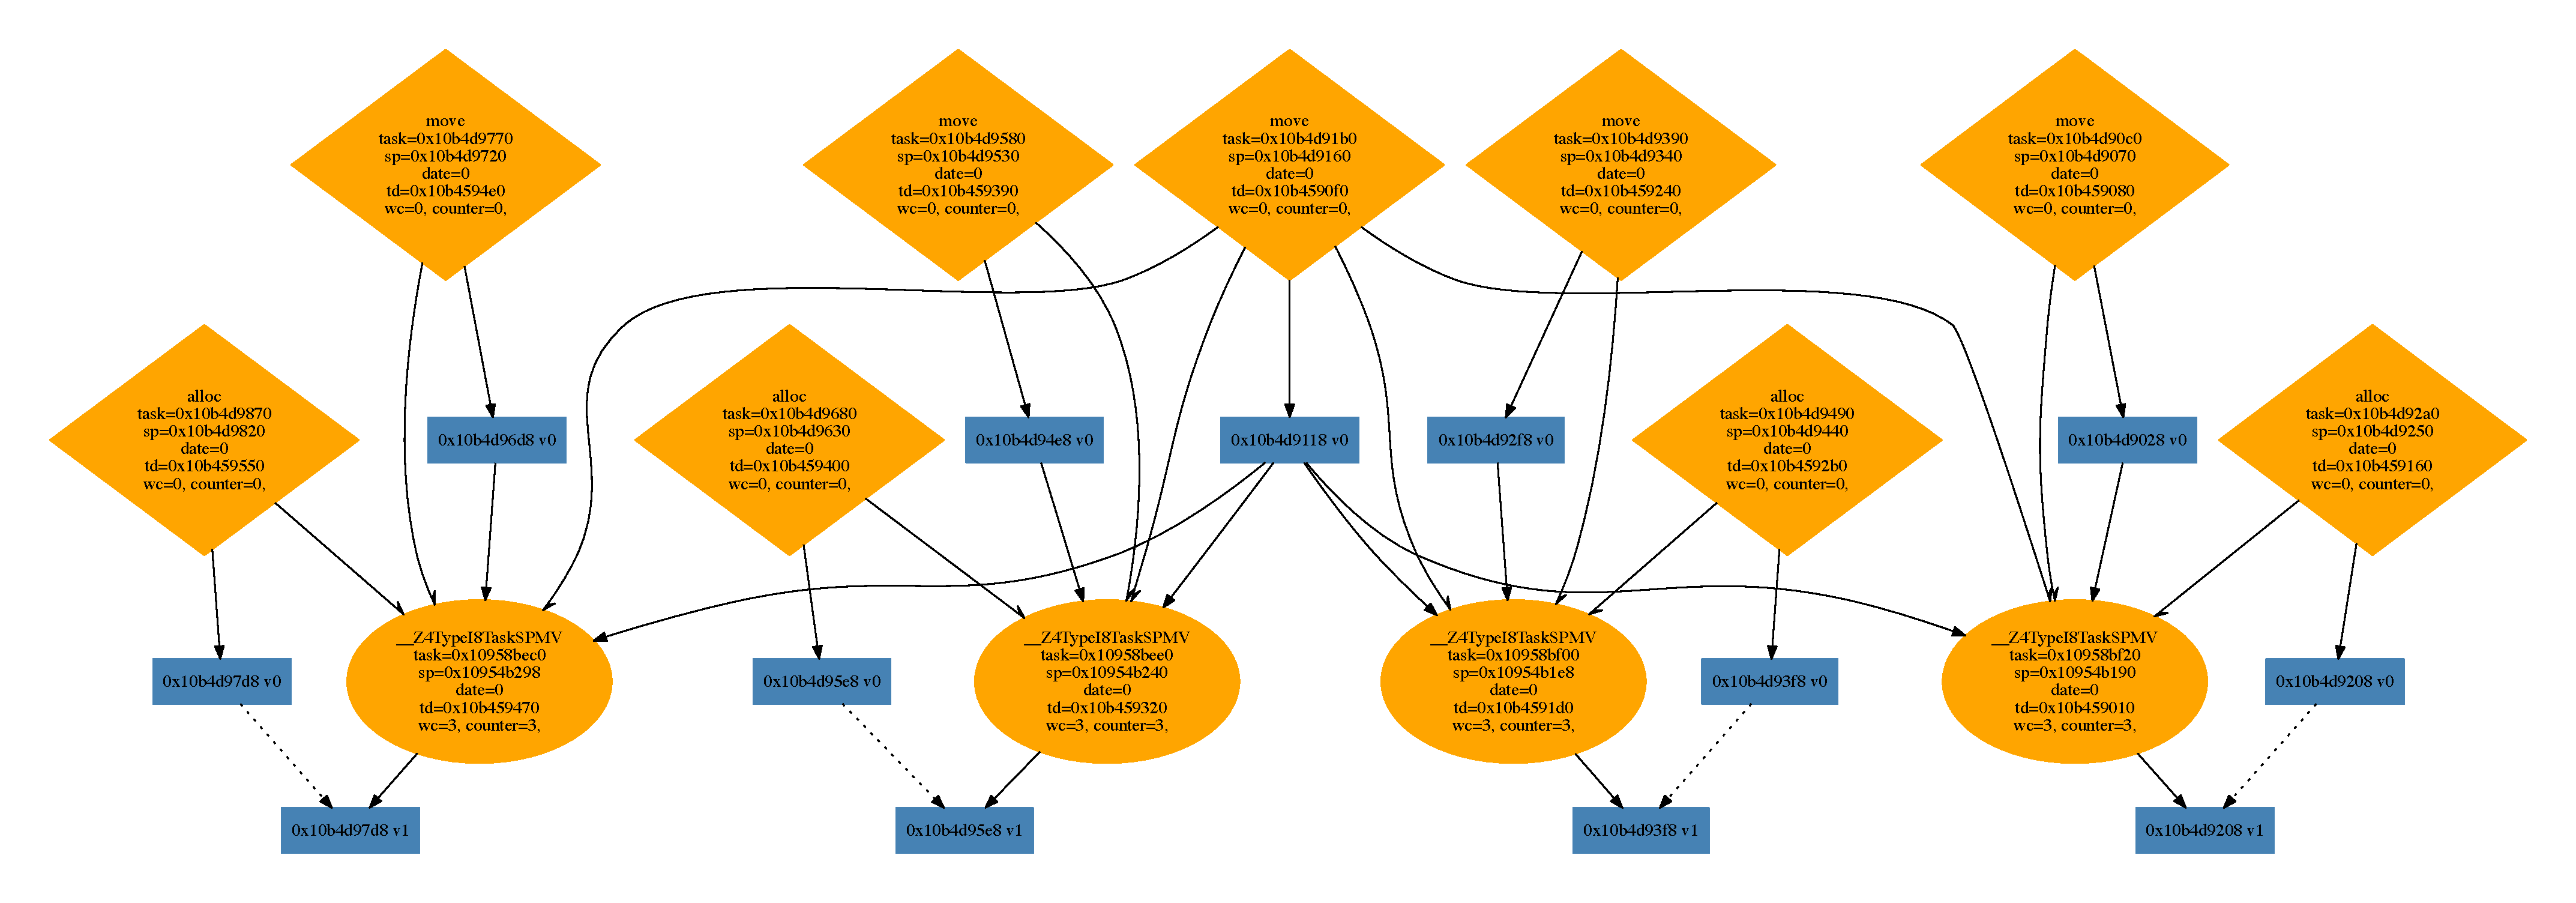
\includegraphics[width=\textwidth]{spmv-2048-512}
  \end{figure}
\end{frame}
%------------------------------------------------------------------------------

%
%%%%%%%%%%%%%%%%%%%%%%%%%%%%%%%%%%%%%%%%%%%%%%%%%%%%%%%%%%%%%%%%%%%%%%%%%%%%%%%
\section{Conclusion}
%%%%%%%%%%%%%%%%%%%%%%%%%%%%%%%%%%%%%%%%%%%%%%%%%%%%%%%%%%%%%%%%%%%%%%%%%%%%%%%

\begin{frame}
  \frametitle{Conclusion}
  \begin{itemize}
  \item Parallel systems are widely used to improve performance on applications. 
    \begin{itemize}
    \item Fluid dynamics and climatological models.
    \end{itemize}
  \pause
  \item Increasing adoption of data dependency.
    \begin{itemize}
    \item OpenMP introduced data dependency in its last version.
    \end{itemize}
  \pause
  \item Still data-flow task programming is a candidate for Exascale systems.
    \begin{itemize}
    \item Many questions remain such as scalability (tasks, graph size).
    \item Few studies on modern distributed systems.
    \end{itemize}
  \end{itemize}
\end{frame}

%%%%%%%%%%%%%%%%%%%%%%%%%%%%%%%%%%%%%%%%%%%%%%%%%%%%%%%%%%%%%%%%%%%%%%%%%%%%%%%%
\section*{References}
%%%%%%%%%%%%%%%%%%%%%%%%%%%%%%%%%%%%%%%%%%%%%%%%%%%%%%%%%%%%%%%%%%%%%%%%%%%%%%%

\begin{frame}
  \frametitle{References}
  \begin{itemize}\footnotesize
  \item {\bf Parallel Architectures: hardware and software evolution}, Vincent Danjean, 2014: 
    \url{http://goo.gl/cZfFdN}
  \item {\bf StarPU Tutorial},  ComPAS 2013: \url{http://goo.gl/1V4jpH}
  \item {\bf Runtime Systems for Heterogeneous Platform Programming}, StarPU tutorial, 2014: \url{http://goo.gl/3YM9IM}
  \item {\bf The OmpSs programming model}: \url{https://pm.bsc.es/ompss}
  \item {\bf XKaapi tutorial} Thierry Gautier, João V. F. Lina. PACT training, 2014:
    \url{http://kaapi.gforge.inria.fr/dokuwiki/doku.php?id=tutorial_bordeaux}
  \end{itemize}
\end{frame}


%------------------------------------------------------------------------------
\begin{frame}[plain]{}
  \begin{center}
    \vspace{2cm}
    \Large{https://joao-ufsm.github.io/par2023a/}
    
    \vspace{1cm}
    
\includegraphics[width=2cm]{logo_ufsm}
    \hspace{0.5cm}
    
\includegraphics[width=2cm]{logo_inf}
  \end{center}
\end{frame}
%------------------------------------------------------------------------------


\end{document}
